% Mémoire de stage de fin d'études — ENSAE Paris, Mastère spécialisé, année 2025-2026
% Compilation : latexmk -xelatex DANTZIKIAN_Alexis_MS25.tex
\documentclass[12pt,a4paper]{article}

\usepackage{amsmath}
\usepackage{fontspec}
\usepackage{unicode-math}
\setmainfont{Times New Roman}
\setmathfont{TeX Gyre Termes Math}
\usepackage[english,french]{babel}
\frenchsetup{og=«, fg=»}
\usepackage[a4paper,margin=2.5cm]{geometry}
\usepackage{setspace}
\onehalfspacing
\usepackage{graphicx}
\usepackage{booktabs}
\usepackage{array}
\usepackage{tabularx}
\usepackage{multirow}
\usepackage{threeparttable}
\usepackage[font=small,labelfont=bf,labelsep=period]{caption}
\usepackage{float}
\usepackage{enumitem}
\usepackage{xcolor}
\usepackage{microtype}
\usepackage{tocloft}
\renewcommand{\cfttoctitlefont}{\Large\bfseries}
\setlength{\cftbeforesecskip}{0.35em}
\usepackage[round,semicolon]{natbib}
\usepackage[hidelinks]{hyperref}

\graphicspath{{figures/}}
\setlength{\parindent}{0pt}
\setlength{\parskip}{0.45em}
\setlist{itemsep=0.15em,topsep=0.3em}
\renewcommand{\arraystretch}{1.1}
\captionsetup[table]{position=top,skip=4pt}

% Éléments que l'auteur doit renseigner : visibles en rouge dans le PDF
\newcommand{\acompleter}[1]{\textcolor{red}{[à compléter : #1]}}

\DeclareMathOperator{\Var}{Var}
\DeclareMathOperator{\Cov}{Cov}
\newcommand{\E}{\mathbb{E}}
\newcommand{\Q}{\mathbb{Q}}
\renewcommand{\P}{\mathbb{P}}
\newcommand{\F}{\mathcal{F}}
\newcommand{\dd}{\mathrm{d}}

\begin{document}

% ---------------------------------------------------------------------------------------------------
% Page de couverture (modèle imposé par les consignes de l'ENSAE, p. 12)
% ---------------------------------------------------------------------------------------------------
\begin{titlepage}
\singlespacing
\noindent
\begin{minipage}[t]{0.48\textwidth}
\textbf{DANTZIKIAN Alexis}
\end{minipage}\hfill
\begin{minipage}[t]{0.48\textwidth}\raggedleft
\textbf{Mastère Spécialisé} \acompleter{nom du mastère spécialisé}
\end{minipage}

\vspace{0.6cm}
\noindent Stage de fin d'études\\
Année scolaire 2025-2026

\vfill
\begin{center}
{\LARGE\bfseries Options européennes sur OAT\\[0.3em] dans un modèle gaussien à deux facteurs\par}
\vspace{0.8cm}
{\large Spread OAT–€STR, identification des paramètres et prix exact\par}
\end{center}
\vfill

\noindent
\begin{minipage}[t]{0.48\textwidth}
\acompleter{nom de l'entreprise}\\
\acompleter{ville}
\end{minipage}\hfill
\begin{minipage}[t]{0.48\textwidth}\raggedleft
Maître de stage : \acompleter{Prénom NOM}\\
\acompleter{dates du stage}
\end{minipage}
\end{titlepage}

% ---------------------------------------------------------------------------------------------------
\renewcommand{\contentsname}{Sommaire}
\setcounter{tocdepth}{2}
\begin{spacing}{1.0}
\tableofcontents
\end{spacing}
\newpage

\section*{Introduction}
\addcontentsline{toc}{section}{Introduction}

\subsection*{Cadre du stage}

Le stage s'est déroulé chez \acompleter{nom de l'entreprise}, au sein de \acompleter{équipe ou desk}, du
\acompleter{dates du stage}, sous la responsabilité de \acompleter{Prénom NOM, fonction}.
\acompleter{missions confiées pendant le stage, en deux ou trois phrases}.

Le présent rapport porte sur l'évaluation d'options européennes sur obligations d'État françaises (OAT). Le
contrat étudié suit les conventions de marché de la banque d'accueil : une option vanille, collatéralisée et
actualisée au taux €STR, dont le prix à terme est fixé par le financement du titre en pension livrée (repo). Les
données de marché proviennent de Bloomberg (clôture du 8 septembre 2026). Les calculs sont programmés en
Python, avec les bibliothèques NumPy, SciPy et pandas pour l'analyse numérique, statsmodels pour le filtre de
Kalman, le modèle à changement de régime et les tests statistiques, et scikit-learn pour l'analyse en
composantes principales. L'annexe~D décrit l'environnement de calcul.

\subsection*{Problématique}

Le rendement d'une OAT n'est pas le taux sans risque. Il s'en écarte d'un spread contre l'€STR qui rémunère le
risque de crédit de l'État, la liquidité du titre et des effets d'offre, et ce spread fluctue en partie
indépendamment des taux. Un pricer d'options sur obligations calibré sur les seules swaptions €STR ignore cette
source de volatilité. Or il n'existe pas de marché liquide d'options sur OAT d'où l'on pourrait la tirer : la
volatilité du spread doit être mesurée ailleurs, et il faut vérifier que les données disponibles le permettent.
Le mémoire pose donc la question suivante :

\begin{center}
\begin{minipage}{0.88\textwidth}
\itshape Faut-il modéliser le spread OAT–€STR comme un facteur de risque à part pour évaluer une option
européenne sur OAT, et peut-on en identifier les paramètres avec les données disponibles ?
\end{minipage}
\end{center}

\subsection*{Littérature et positionnement}

Le cadre retenu est le modèle gaussien à deux facteurs additifs, dit G2++, de \citet{BrigoMercurio2006}
(section~4.2), qui étend le modèle de \citet{HullWhite1990}. Le modèle recale exactement la courbe initiale, et
une option sur obligation à coupons y a un prix exact sous forme d'intégrale à une dimension (théorème~4.2.3).
À un facteur, la décomposition de \citet{Jamshidian1989} ramène cette option à une somme d'options sur
zéro-coupons. \citet{Russo} lisent le second facteur du G2++ comme un spread de crédit : le premier facteur
décrit le taux sans risque, le second l'écart entre la courbe risquée et la courbe sans risque. Ils remplacent
le prix exact par une formule fermée approchée, sous une hypothèse lognormale à «~poids gelés~», et proposent de
calibrer le facteur spread sur la seule courbe risquée.

Cette forme du taux d'actualisation se justifie dans les modèles de crédit à intensité
\citep{DuffieSingleton1999}, et \citet{MonfortRenne2014} l'appliquent aux souverains de la zone euro en séparant
crédit et liquidité ; seul le spread total entre toutefois dans le prix d'une option sur OAT.

Le travail reprend le modèle de \citet{Russo} sur des données françaises, avec trois différences. Le contrat
est celui qui se traite en banque, avec un forward fixé par le repo et non par le modèle. Le prix est calculé
exactement, à partir du théorème~4.2.3 de \citet{BrigoMercurio2006} adapté à deux courbes, et l'approximation à
poids gelés est mesurée contre lui. Enfin, l'identification des paramètres du spread est testée avant leur
estimation : la procédure de calibration du papier se révèle non identifiante, et l'estimation se fait sur les
séries historiques.

\subsection*{Hypothèses testées}

La question se décompose en cinq hypothèses, résumées au tableau~\ref{tab:hypotheses} ; la conclusion dit
pour chacune si elle est confirmée.

\begin{table}[htbp]
\centering\small
\caption{Hypothèses du mémoire et tests associés}
\label{tab:hypotheses}
\begin{tabularx}{\textwidth}{@{}l X X c@{}}
\toprule
 & Hypothèse & Test & Section \\
\midrule
H1 & La courbe OAT identifie les paramètres du facteur spread (procédure de Russo et al.) & forme de l'objectif de calibration & 5.1 \\
H2 & Les séries historiques identifient ces paramètres, sous la mesure de pricing comme sous la mesure historique & méthode des moments généralisée, régimes, filtre de Kalman, données simulées & 5, 6 \\
H3 & Le facteur spread renchérit sensiblement l'option par rapport au seul facteur taux & prix à la monnaie, décomposition de la variance, volatilités réalisées & 7.2 \\
H4 & Cet effet exige deux facteurs, et pas seulement une volatilité plus forte & comparaison à un Hull-White à un facteur équivalent & 7.3 \\
H5 & L'approximation à poids gelés de Russo et al. suffit pour le pricing & comparaison au prix exact, validé par Monte-Carlo & 7.1 \\
\bottomrule
\end{tabularx}
\end{table}

\subsection*{Enseignements de l'ENSAE mobilisés}

Trois cours de l'ENSAE fondent les choix du mémoire. Le pricing de taux s'appuie sur le cours de
\citet{Chaix2021} (actualisation au taux du collatéral, mesure forward, volatilité normale des swaptions,
Hull-White à un facteur et sa calibration sur une diagonale de swaptions) et sur celui de \citet{Hillairet2026}
(construction de la courbe, modèles de taux court à shift déterministe, probabilité forward, décomposition de
Jamshidian). L'estimation s'appuie sur le cours de \citet{MPR2025} : modèles affines gaussiens et changement de
mesure (cours~1 et~3), relation forward d'un actif stockable (cours~2), régimes de Markov (cours~4), méthode des
moments généralisée, filtre de Kalman, problème de persistance et pricing des risques de crédit et de liquidité
(cours~5). Les renvois précis, au chapitre ou à la page, figurent dans le texte.

\subsection*{Part du travail personnel}

\acompleter{rôle du maître de stage et de l'équipe : choix du sujet, données fournies, conventions de marché,
relectures ; part personnelle de l'élève dans la modélisation, la programmation et l'analyse}. La courbe de
repo, faute de cotations accessibles, est fictive et signalée comme telle à chaque usage ; la section~7 mesure
l'effet de son niveau sur les prix.

\subsection*{Plan}

La section~1 présente les données et construit les deux courbes, €STR et OAT. La section~2 expose le modèle à
deux facteurs et justifie la lecture du second facteur comme un spread. La section~3 définit le contrat, le
forward repo et le recentrage du modèle sur ce forward, puis établit le prix exact et l'approximation à poids
gelés. Les sections~4 à~6 traitent de la calibration : le facteur taux sur les swaptions, puis le facteur
spread, dont on montre d'abord que la courbe OAT ne l'identifie pas, avant de l'estimer par la méthode des
moments généralisée et par maximum de vraisemblance avec filtre de Kalman. La section~7 valide le prix exact et
présente les résultats, hypothèse par hypothèse. La conclusion reprend les réponses, les limites et les
prolongements possibles.

\section{Données et courbes de marché}
\label{sec:donnees}

\subsection{Données}

Les données de marché sont celles de Bloomberg à la clôture du 8 septembre 2026, pour un règlement le
10 septembre. Cette date de règlement est l'origine des temps, $t=0$ ; le temps est mesuré en années sur une base
ACT/365, sans calendrier de jours ouvrés. Le tableau~\ref{tab:donnees} décrit les quatre sources utilisées.

\begin{table}[htbp]
\centering\small
\caption{Données de marché (Bloomberg, clôture du 8 septembre 2026)}
\label{tab:donnees}
\begin{tabularx}{\textwidth}{@{}l X X@{}}
\toprule
Source & Contenu & Usage \\
\midrule
Courbe €STR & 32 taux de swaps OIS €STR, de 1 semaine à 50 ans & courbe sans risque \\
Cube de swaptions & volatilités normales des swaptions EUR à la monnaie, 21 expiries $\times$ 14 tenors & calibration du facteur taux \\
OAT & 19 titres d'État (5 zéro-coupons courts, 14 OAT de 2028 à 2072) : coupon, maturité, prix clean & courbe OAT, sous-jacent \\
Historiques & rendements OAT génériques et taux de swaps €STR à 2, 5, 10, 15, 20, 25 et 30 ans, quotidiens & estimation du facteur spread \\
\bottomrule
\end{tabularx}
\end{table}

Les historiques couvrent la période du 1\textsuperscript{er} janvier 2021 au 8 septembre 2026, soit 1\,475 jours
ouvrés. Ils sont exportés avec des dates mal formées, dates Excel et texte au format américain mêlés ; la grille
étant quotidienne et complète, on la reconstruit. Les séries s'arrêtent à la date de valorisation, de sorte
qu'aucune information postérieure n'entre dans l'estimation.

S'y ajoute une courbe de spread repo, écart entre le taux de pension livrée de l'OAT et le taux zéro €STR de même
durée. Faute de cotations accessibles, \emph{cette courbe est fictive} : elle vaut +20~pb à trois semaines, puis
croît linéairement jusqu'à +75~pb à dix ans. Les options étudiées ont une échéance de dix ans au plus, de sorte
que la courbe couvre toutes les échéances sans jamais être prolongée. Une courbe de marché la remplacerait au même
format, sans modification du code ; la section~\ref{sec:resultats} mesure l'effet de son niveau.

\begin{figure}[htbp]
\centering
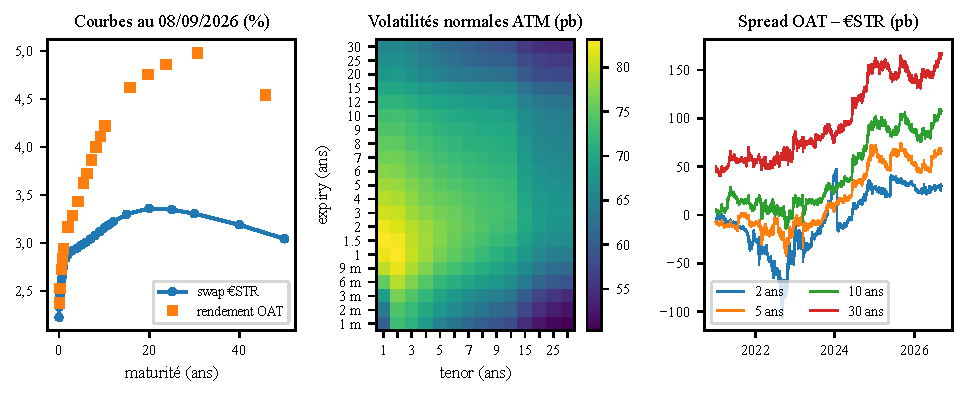
\includegraphics[width=\textwidth]{donnees}
\caption{Données au 8 septembre 2026. À gauche, taux de swaps €STR et rendements des OAT ; au centre,
volatilités normales des swaptions à la monnaie ; à droite, historique du spread OAT–€STR à quatre tenors.}
\label{fig:donnees}
\end{figure}

La figure~\ref{fig:donnees} résume ces données. Aux tenors longs, le spread OAT–€STR s'est élargi d'une
centaine de points de base depuis 2021, avec deux sauts nets, en juin 2024 puis à l'automne 2024. À deux ans, il est resté négatif presque
tout au long de 2021 et 2022.

\subsection{Courbe sans risque €STR}

Les swaps OIS €STR, qui ont remplacé les swaps EONIA \citep[CM1, p.~12]{Hillairet2026}, servent à construire la
courbe sans risque $P^M(0,T)$. Le taux OIS est le rendement du seul taux court au jour le jour
\citep[cours~5, éq.~II.17]{MPR2025}, et la même courbe actualise les flux collatéralisés
\citep[section~3.4]{Chaix2021}. Un swap de maturité $T$ et de taux fixe $S$, à jambe fixe annuelle, vaut zéro à
l'initiation :
\begin{equation}
S \sum_{i} \tau_i\,P^M(0,T_i) + P^M(0,T) = 1, \qquad T_i = T, T-1, \dots
\end{equation}
On résout cette équation pilier après pilier (\emph{bootstrap}), $P^M(0,T)$ étant la seule inconnue une fois
les facteurs d'actualisation intermédiaires interpolés linéairement en taux zéro. La courbe obtenue reprice
les 32 swaps à 0,25~pb près.

Le modèle utilise le forward instantané $f^M(0,t) = -\partial_t \log P^M(0,t)$, qui entre dans le terme de
recalage. Une interpolation linéaire des taux zéro donnerait un forward discontinu ; on interpole donc
$\log P^M(0,T)$ par une spline cubique, ce qui rend $f^M$ continu et dérivable. La courbe €STR étant
décroissante au-delà de vingt ans, le forward long y est nettement inférieur aux taux zéro : environ 1,4~\%
à cinquante ans, pour un taux zéro proche de 2,8~\%.

\subsection{Courbe OAT et sous-jacent}

La courbe $\bar P^M(0,T)$ est la courbe d'actualisation qui reprice les OAT. Un bootstrap titre par titre
propagerait à toute la courbe l'erreur de prix du titre le plus court et dépendrait des particularités de chaque
titre \citep[CM1, p.~27]{Hillairet2026}, alors que le modèle a besoin d'un forward régulier. On ajuste donc la
paramétrisation de \citet{NelsonSiegel1987} étendue par \citet{Svensson1994}, qu'utilisent la plupart des
banques centrales \citep[cours~3, slide~109]{MPR2025}, sur le taux zéro continu :
\begin{equation}
\begin{split}
\bar R(T) = \beta_0 + \beta_1\,\frac{1-e^{-T/\lambda_1}}{T/\lambda_1}
&+ \beta_2\Big(\frac{1-e^{-T/\lambda_1}}{T/\lambda_1} - e^{-T/\lambda_1}\Big)
+ \beta_3\Big(\frac{1-e^{-T/\lambda_2}}{T/\lambda_2} - e^{-T/\lambda_2}\Big), \\
\bar P^M(0,T) &= e^{-\bar R(T)\,T}.
\end{split}
\end{equation}
Les six paramètres sont ajustés par moindres carrés sur les prix dirty (coupon couru inclus) des dix-neuf
titres. Chaque erreur de prix est divisée par la duration du titre, ce qui la rend homogène à une erreur de
rendement ; sans cette pondération, les titres longs domineraient l'ajustement. Le coupon couru, calculé en
ACT/ACT, sert à passer du prix clean (pied de coupon) au prix dirty, aujourd'hui comme à l'échéance d'une
option.

L'erreur quadratique moyenne est de 4,1~pb de rendement (annexe~C). Les résidus se concentrent sur l'extrême long
terme, que six paramètres ne peuvent pas reproduire : les OAT 2050 (coupon de 1,5~\%) et 2072 (0,5~\%) se
traitent cher, par demande de duration et de convexité, et l'OAT 2057 sous la courbe (résidu de $-14{,}5$~pb). Ces
écarts pèsent peu sur le prix de l'option. Son forward est calculé à partir du prix de marché du sous-jacent
(section~\ref{sec:evaluation}), et la courbe OAT n'y entre qu'à travers la répartition des flux et la loi du
spread.

\begin{figure}[htbp]
\centering
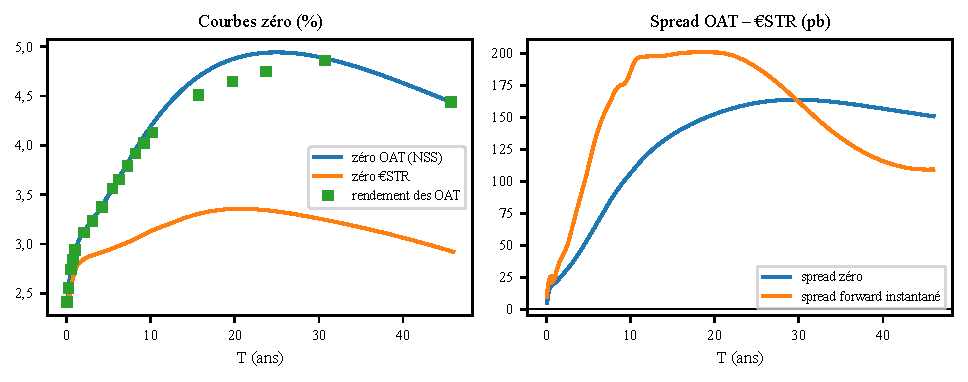
\includegraphics[width=\textwidth]{courbe_oat}
\caption{Courbes zéro OAT (Nelson-Siegel-Svensson) et €STR, et spread OAT–€STR en taux zéro et en taux forward
instantané.}
\label{fig:courbe_oat}
\end{figure}

Le spread zéro $\bar R(T) - R(T)$ et le spread forward $\bar f^M - f^M$ de la figure~\ref{fig:courbe_oat}
donnent la partie déterministe du facteur spread. Le spread court est faible : le taux OAT contient, outre le
risque de défaut, des primes de liquidité et de collatéral \citep[p.~8]{Russo}, et le spread peut changer de
signe, comme à deux ans en 2021-2022. Un modèle gaussien, où le spread n'est pas contraint à rester positif, est
donc admissible.

Les options portent sur l'OAT 4,10~\% du 25 mai 2046 (FR0014015MU5), de maturité résiduelle 19,7 ans, dont le
prix clean est 91,690 et le prix dirty 92,903. La courbe la reprice à 2,0~pb de rendement près. Les échéances
des options sont 1, 2, 5, 7 et 10 ans ; à dix ans, il reste encore dix flux au titre.

\section{Un modèle gaussien à deux facteurs pour le taux OAT}
\label{sec:modele}

\subsection{Dynamique et moments gaussiens}

Le taux court sans risque s'écrit $r(t) = \alpha(t) + x(t)$ et le spread court OAT–€STR
$s(t) = \beta(t) + y(t)$, où $\alpha$ et $\beta$ sont déterministes et où $x$ et $y$ sont deux processus
d'Ornstein-Uhlenbeck centrés \citep[éq.~4.4-4.5]{BrigoMercurio2006} :
\begin{equation}
\dd x = -a_x\,x\,\dd t + \sigma_x\,\dd W_x,\qquad \dd y = -a_y\,y\,\dd t + \sigma_y\,\dd W_y,\qquad
\dd W_x\,\dd W_y = \rho\,\dd t,
\label{eq:dynamique}
\end{equation}
avec $x(0) = y(0) = 0$.
Le taux court de l'OAT est $\bar r = r + s = \bar\alpha + x + y$, avec $\bar\alpha = \alpha + \beta$. Dans les
notations de \citet{BrigoMercurio2006}, $(a_x, a_y, \sigma_x, \sigma_y)$ sont $(a, b, \sigma, \eta)$ et
$\bar\alpha$ est $\varphi$.

Toutes les formules du modèle se ramènent aux moments, conditionnels à $\F_t$, du vecteur gaussien formé de
$x(T)$, $y(T)$, $\int_t^T x$ et $\int_t^T y$. Avec $\tau = T - t$, la duration stochastique d'un zéro-coupon est
\begin{equation}
H_a(t,T) = \frac{1-e^{-a\tau}}{a}, \qquad \E\Big[\int_t^T x(u)\,\dd u \,\Big|\, \F_t\Big] = H_{a_x}(t,T)\,x(t),
\end{equation}
et la variance de l'intégrale d'un facteur de paramètres $(a,\sigma)$ vaut
\begin{equation}
V_{a,\sigma}(t,T) = \Var\Big[\int_t^T x(u)\,\dd u\Big]
= \frac{\sigma^2}{a^2}\Big[\tau + \frac{2}{a}e^{-a\tau} - \frac{1}{2a}e^{-2a\tau} - \frac{3}{2a}\Big].
\end{equation}
Le terme croisé est deux fois la covariance des intégrales \citep[lemme~4.2.1, éq.~4.10]{BrigoMercurio2006} :
\begin{equation}
V_{xy}(t,T) = \frac{2\rho\sigma_x\sigma_y}{a_x a_y}\Big[\tau - H_{a_x}(t,T) - H_{a_y}(t,T)
+ \frac{1-e^{-(a_x+a_y)\tau}}{a_x+a_y}\Big],
\end{equation}
et la variance totale $\bar V = V_x + V_y + V_{xy} = \Var\big[\int_t^T (x+y)\big]$ est la variance $V(t,T)$ du
livre. Les variances et covariances des facteurs eux-mêmes, qui servent au pricing, sont données en annexe~A.

\subsection{Le facteur taux seul : Hull-White et Jamshidian}

Lorsque $\sigma_y = 0$, le modèle se réduit à celui de Hull et White sous la forme $r = \alpha + x$
\citep[section~3.3]{BrigoMercurio2006}. Le terme déterministe recale la courbe €STR :
$\int_0^T \alpha = -\log P^M(0,T) + \tfrac12 V_x(0,T)$. Comme $\int_t^T x$ est gaussien de moyenne
$H_{a_x}(t,T)\,x(t)$ et de variance $V_x(t,T)$, le prix d'un zéro-coupon est log-affine en $x(t)$
\citep[éq.~3.39]{BrigoMercurio2006} :
\begin{equation}
P(t,T) = \frac{P^M(0,T)}{P^M(0,t)}\,\exp\Big(-H_{a_x}(t,T)\,x(t) + \tfrac12\big[V_x(t,T) - V_x(0,T) + V_x(0,t)\big]\Big).
\label{eq:zc_hw}
\end{equation}

Une option européenne d'échéance $T_0$ et de strike $X$ sur une obligation de flux $K_i$ aux dates $T_i$ a, dans
ce modèle, un prix exact. Le prix de l'obligation en $T_0$ étant décroissant en $x(T_0)$, il existe un unique
$x^\ast$ tel que $\sum_i K_i P(T_0,T_i;x^\ast) = X$, et l'option se décompose en une somme d'options sur
zéro-coupons de strikes $X_i = P(T_0,T_i;x^\ast)$, chacune de formule fermée \citep{Jamshidian1989} ;
\citet[section~3.11.1]{BrigoMercurio2006} et \citet[section~6.3.6]{Chaix2021} en donnent la mise en œuvre. Une
swaption payeuse est un put de strike 1 sur l'obligation formée de la jambe fixe et du nominal : elle se price de
la même façon \citep[éq.~3.44-3.46]{BrigoMercurio2006}. À la monnaie, son prix de marché en volatilité normale
$\sigma_N$ est $A\,\sigma_N\sqrt{T_0/2\pi}$, où $A$ est l'annuité du swap sous-jacent.

\subsection{Le spread comme second facteur}

\citet{Russo} lisent les deux facteurs du G2++ comme le taux sans risque et le spread de crédit. On modélise ici
directement le spread court OAT–€STR. Il contient la prime de crédit de l'État français, mais aussi des primes de
liquidité et de collatéral : il est traité comme un facteur de risque de marché, sans chercher à en isoler la part
de défaut.

Les modèles de crédit à intensité justifient la forme $\bar r = r + y$. Supposons que le défaut soit un état
absorbant, qu'il ne cause pas les facteurs de taux, lesquels ne sautent pas au défaut, et que l'événement de
défaut lui-même ne soit pas pricé. Avec un recouvrement en valeur de marché, où le porteur récupère au défaut une
fraction $\zeta$ du prix qu'aurait eu le titre sans défaut, le prix avant défaut d'un zéro-coupon risqué est
\begin{equation}
\bar P(t,T) = \E^{\Q}_t\Big[e^{-\int_t^T (r_u + \tilde\lambda_u)\,\dd u}\Big],\qquad \tilde\lambda \approx (1-\zeta)\,\lambda,
\end{equation}
où $\lambda$ est l'intensité de défaut et $\tilde\lambda$ l'intensité ajustée du recouvrement
\citep[cours~5, hypothèses~II.1-II.3 et prop.~II.1-II.2]{DuffieSingleton1999,MPR2025}. Les prix ne
révèlent que le produit de la perte et de l'intensité, jamais l'une sans l'autre, et une prime de liquidité
s'ajoute de la même façon au taux d'actualisation (éq.~II.15 du cours). \citet[section~22.4]{BrigoMercurio2006}
écrivent la même forme pour un recouvrement nul et une intensité corrélée aux taux. Le spread total $s = \beta + y$
est donc modélisé par un facteur gaussien sans paramètre de perte : $y$ est une intensité ajustée qui agrège
crédit, liquidité et collatéral. Ce cadre fonde la forme du taux d'actualisation avant défaut ; le mémoire ne
modélise ni la date de défaut ni le saut du prix au défaut.

Le terme $\bar\alpha$ recale directement la courbe OAT \citep[corollaire~4.2.1, éq.~4.13]{BrigoMercurio2006} :
\begin{equation}
\int_0^T\bar\alpha(u)\,\dd u = -\log\bar P^M(0,T) + \tfrac12\bar V(0,T),
\label{eq:recalage}
\end{equation}
et la différence $\bar\alpha - \alpha = \beta$ est le spread forward de marché augmenté des termes de convexité du
spread et du terme croisé. Comme $\int_t^T(x+y)$ est gaussien de moyenne $H_{a_x}x(t) + H_{a_y}y(t)$ et de
variance $\bar V(t,T)$, le zéro-coupon OAT vaut \citep[théorème~4.2.1]{BrigoMercurio2006}
\begin{equation}
\bar P(t,T) = \frac{\bar P^M(0,T)}{\bar P^M(0,t)}\exp\Big(-H_{a_x}(t,T)\,x(t) - H_{a_y}(t,T)\,y(t)
+ \tfrac12\big[\bar V(t,T) - \bar V(0,T) + \bar V(0,t)\big]\Big).
\label{eq:zc_oat}
\end{equation}
C'est l'expression des équations~16 à~24 de \citet{Russo}. Une OAT de flux $K_i$ aux dates $T_i$ vaut
$\bar B(t) = \sum_i K_i \bar P(t,T_i)$ (prix dirty), et ses durations stochastiques sont
$D_x = \sum_i w_i H_{a_x}(t,T_i)$ et $D_y = \sum_i w_i H_{a_y}(t,T_i)$, avec $w_i = K_i\bar P(t,T_i)/\bar B(t)$.
Lorsque les deux vitesses de retour sont faibles, $H_{a_x} \approx H_{a_y}$ : les deux facteurs déplacent alors
les prix des OAT de la même façon, propriété qui reviendra à la section~\ref{sec:resultats}.

\section{Évaluation de l'option sur OAT}
\label{sec:evaluation}

\subsection{Le contrat}

L'option européenne d'échéance $T_0$ et de strike $K$, exprimé sur le prix clean, paie
$\big(\bar B^{clean}(T_0) - K\big)^+$ pour un call et $\big(K - \bar B^{clean}(T_0)\big)^+$ pour un put. Le
coupon couru $CC(T_0)$ à l'échéance est connu dès aujourd'hui, si bien que
$\bar B^{clean}(T_0) - K = \bar B(T_0) - X$ avec le strike dirty $X = K + CC(T_0)$ : le modèle travaille sur le
prix dirty, somme actualisée des flux. L'option est collatéralisée et actualisée au taux €STR. Sous la mesure
$T_0$-forward €STR $\Q^{T_0}$, de numéraire $P(\cdot,T_0)$ \citep[CM3]{Hillairet2026}, son prix est
\begin{equation}
C = P(0,T_0)\,\E^{T_0}\big[(\bar B(T_0) - X)^+\big].
\label{eq:prix_call}
\end{equation}
Les strikes sont exprimés en pourcentage du forward clean défini ci-dessous, et les prix en pourcentage du nominal.

\subsection{Le forward repo}

Acheter l'OAT au prix dirty de marché $\bar B^M(0)$, la financer en repo jusqu'en $T_0$ et rembourser le
financement avec les coupons encaissés d'ici là permet de livrer le titre en $T_0$. Par absence d'arbitrage, le
prix forward dirty est
\begin{equation}
F = \frac{\bar B^M(0) - \sum_{0 < T_i \le T_0} K_i\,P^{repo}(0,T_i)}{P^{repo}(0,T_0)},\qquad
P^{repo}(0,T) = P^M(0,T)\,e^{-s^{repo}(T)T},
\label{eq:forward}
\end{equation}
où $s^{repo}(T)$ est le spread du taux repo zéro continu contre l'€STR. Un contrat forward collatéralisé en €STR
a pour prix d'équilibre $\E^{T_0}[\bar B(T_0)]$. Comme l'écart entre repo et €STR est déterministe, le portage se
réplique, et $\E^{T_0}[\bar B(T_0)] = F$. C'est la relation forward d'un actif stockable
\citep[cours~2, slides~16-18]{MPR2025} : vu de l'€STR, le spread repo est l'opposé d'un rendement d'opportunité
(\emph{convenience yield}), qui serait positif pour un titre «~spécial~» en repo. Le forward clean, auquel on
rapporte les strikes, est $F^{clean} = F - CC(T_0)$, et la parité call-put s'écrit
$C - \text{Put} = P(0,T_0)\,(F^{clean} - K)$.

Le forward n'utilise le spread repo qu'aux dates antérieures à l'échéance : la courbe repo doit couvrir $T_0$.
Elle est définie jusqu'à dix ans, la plus longue échéance étudiée, et n'est jamais prolongée, de sorte qu'aucun
prix ne repose sur une extrapolation du financement.

\subsection{Recentrer le modèle sur le forward repo}

Laissé à lui-même, le modèle fait croître le prix de l'OAT au taux $\bar r$ en moyenne. Son espérance forward
s'écrit
\begin{equation}
\begin{split}
M &= \sum_{T_i>T_0} m_i,\\
m_i &= K_i\,\E^{T_0}\big[\bar P(T_0,T_i)\big]
= K_i A_i\exp\Big(-H_x^i\mu_x - H_y^i\mu_y + \tfrac12\Var\big(H_x^i x(T_0) + H_y^i y(T_0)\big)\Big),
\end{split}
\end{equation}
où $A_i$ est la partie déterministe de $\bar P(T_0,T_i)$ dans~\eqref{eq:zc_oat}, $H^i_\cdot = H_{a_\cdot}(T_0,T_i)$,
et $(\mu_x,\mu_y)$ les moyennes de $(x(T_0),y(T_0))$ sous $\Q^{T_0}$. Comme dans
\citet[lemme~4.2.2]{BrigoMercurio2006}, le changement de numéraire ajoute à la dérive des facteurs leur covariance
avec le numéraire. Celui-ci est ici le zéro-coupon €STR, qui ne dépend que de $x$ ; en intégrant,
\begin{equation}
\mu_x = -\frac{\sigma_x^2}{2a_x^2}\big(1-e^{-a_xT_0}\big)^2,\qquad
\mu_y = -\frac{\rho\sigma_x\sigma_y}{a_x}\Big[\frac{1-e^{-a_yT_0}}{a_y} - \frac{1-e^{-(a_x+a_y)T_0}}{a_x+a_y}\Big],
\end{equation}
soit $-\Cov\big(x(T_0),\int_0^{T_0}x\big)$ et $-\Cov\big(y(T_0),\int_0^{T_0}x\big)$ ; variances et covariance
sont inchangées.

Le porteur finance l'OAT au taux repo, et non à son propre taux : $M$ ne coïncide pas avec $F$, et l'écart croît
avec $T_0$ comme le portage accumulé. On recale donc le modèle sur le marché, comme $\bar\alpha$ recale la
courbe, en décalant la moyenne du facteur spread en $T_0$ d'une constante $\delta$ telle que
\begin{equation}
\sum_{T_i>T_0} m_i(\delta) = F,\qquad m_i(\delta) = m_i\,e^{-H_y^i\,\delta}.
\label{eq:recentrage}
\end{equation}
$\delta$ s'obtient par une résolution numérique à une dimension d'une expression fermée.

À un terme de convexité près, $\delta$ est nul quand le spread repo égale le spread de l'OAT : le portage est
alors celui de la courbe OAT, et $M = F$. Quand le spread repo est plus faible, le porteur financé en repo
encaisse un portage positif que la diffusion ne justifie pas. Sur un marché sans arbitrage, ce portage rémunère
ce que le modèle gaussien ne contient pas : la perte qu'un événement de crédit ou de liquidité infligerait au
porteur, ou des coûts de financement que le taux repo ne montre pas (décotes, coût de bilan). $F$ est alors
l'espérance du prix y compris cette perte, $M$ son espérance sur une trajectoire sans événement, et $\delta$ fait
passer de l'une à l'autre. L'approximation porte sur la loi : la moyenne du prix intègre la perte anticipée, sa
dispersion non, puisque la loi de $\bar B(T_0)$ reste celle d'un modèle gaussien, sans saut. Son effet reste limité tant que
$\delta$ est petit, ce que la section~\ref{sec:resultats} vérifie pour la courbe repo retenue.

\subsection{Prix exact}

Sous $\Q^{T_0}$, $\big(x(T_0), y(T_0)\big)$ est gaussien, de moyennes $(\mu_x, \mu_y + \delta)$, d'écarts-types
$(s_x, s_y)$ et de corrélation $r_{xy}$ (annexe~A). Le prix de l'OAT à l'échéance est une somme d'exponentielles
affines, $\bar B(T_0) = \sum_i K_iA_i\,e^{-H_x^i x(T_0) - H_y^i y(T_0)}$, décroissante en chaque facteur.
\citet[théorème~4.2.3]{BrigoMercurio2006} en tirent le prix exact d'une swaption, c'est-à-dire d'une option sur
obligation à coupons, sous forme d'intégrale à une dimension. On l'adapte en conditionnant par le facteur spread.
Sachant $y(T_0) = y$, $x(T_0)$ est gaussien de moyenne $m(y) = \mu_x + r_{xy}\,s_x\,(y - \mu_y - \delta)/s_y$ et
d'écart-type $s = s_x\sqrt{1 - r_{xy}^2}$, et le call est exercé si $x(T_0) < x^\ast(y)$, où $x^\ast(y)$ est
l'unique solution de $\bar B(T_0) = X$. Il vient
\begin{equation}
\begin{split}
C &= P(0,T_0)\int_{\mathbb R}\Big[\sum_i K_iA_i\,e^{-H_y^i y - H_x^i m(y) + \frac12 (H_x^i s)^2}\,\Phi\big(d(y) + H_x^i s\big)
- X\,\Phi\big(d(y)\big)\Big]\,\varphi_y(y)\,\dd y,\\
d(y) &= \frac{x^\ast(y) - m(y)}{s},
\end{split}
\label{eq:prix_exact}
\end{equation}
où $\varphi_y$ est la densité de $y(T_0)$ et $\Phi$ la fonction de répartition de la loi normale centrée réduite ;
le put s'obtient en remplaçant le crochet par $X\,\Phi(-d) - \sum_i(\cdots)\,\Phi(-d - H_x^i s)$. L'intégrale est
calculée par quadrature de Gauss-Hermite, et $x^\ast$ par la méthode de Newton sur $\log\bar B$. À $y$ fixé, on
retrouve la décomposition de Jamshidian : les zéro-coupons OAT sont des fonctions décroissantes du seul facteur
$x$, hypothèse sous laquelle \citet[CM3, p.~40-43]{Hillairet2026} l'établit dans un modèle HJM gaussien.

Le prix~\eqref{eq:prix_exact} adapte le théorème du livre sur trois points : il fait intervenir deux courbes
(l'actualisation €STR ne dépend que de $x$, l'OAT de $x + y$), les moyennes forward qui en découlent et le
recentrage $\delta$. Le livre intègre sur le premier facteur ; on intègre sur le second, ce qui garde l'intégrande
régulier quand $\sigma_y$ tend vers zéro et couvre ainsi le cas limite à un facteur, où le prix est celui de
Jamshidian.

\subsection{Approximation à poids gelés}

\citet{Russo} remplacent cette intégrale par une formule fermée, qui étend au G2++ l'approximation proposée à
un facteur par \citet{RussoFabozzi2016}. Si l'on gèle les poids $w_i$ des flux,
$\log\bar B(T_0) \approx c - \bar D_x\,x(T_0) - \bar D_y\,y(T_0)$ est gaussien, de variance
\begin{equation}
\bar\Sigma_B^2 = \bar D_x^2\,\Var x(T_0) + \bar D_y^2\,\Var y(T_0) + 2\bar D_x\bar D_y\,\Cov\big(x(T_0),y(T_0)\big),
\qquad \bar D_\cdot = \sum_{T_i>T_0} w_i\,H_\cdot(T_0,T_i),
\label{eq:sigma_b}
\end{equation}
et de moyenne fixée par $\E^{T_0}[\bar B(T_0)] = F$. \citet{Russo} écrivent cette variance comme une intégrale
évaluée numériquement ; avec des poids gelés, elle est fermée. Ils gèlent les poids à leur valeur d'aujourd'hui ;
on les gèle à leur valeur forward recentrée, $w_i = m_i(\delta)/F$, poids moyen de chaque flux dans le prix de
l'OAT à l'échéance. Le prix approché est alors celui de Black sur le forward repo :
\begin{equation}
C \approx P(0,T_0)\big[F\,\Phi(d_1) - X\,\Phi(d_2)\big],\qquad
d_{1,2} = \frac{\log(F/X) \pm \tfrac12\bar\Sigma_B^2}{\bar\Sigma_B}.
\label{eq:black}
\end{equation}
Cette formule serait exacte si le prix forward de l'OAT était une martingale lognormale sous $\Q^{T_0}$
\citep[CM3, p.~28]{Hillairet2026}. C'est le cas de chaque zéro-coupon, pas de leur somme : l'approximation est
bonne au centre de la distribution et se dégrade dans ses queues (section~\ref{sec:resultats}). Elle garde une
utilité même si l'on dispose du prix exact, car la décomposition de $\bar\Sigma_B^2$ en une part taux, une part
spread et une part croisée, de signe celui de $\rho$, sert à lire les résultats.

\section{Calibration du facteur taux}
\label{sec:taux}

\subsection{Objectif et jeux de calibration}

Comme \citet[section~4.2.7]{BrigoMercurio2006} et \citet[éq.~55]{Russo}, on minimise les écarts relatifs entre
les prix du modèle et les prix de marché de $N$ swaptions à la monnaie :
\begin{equation}
\min_{a_x,\sigma_x}\ \sqrt{\sum_{i=1}^{N}\Big(\frac{\mathit{Swpt}_i(a_x,\sigma_x) - \mathit{Swpt}_i^M}{\mathit{Swpt}_i^M}\Big)^2}.
\end{equation}
Les prix de marché sont les prix de Bachelier ; les prix du modèle sont les prix exacts de Jamshidian. Comme le
prix d'une swaption à la monnaie est linéaire en volatilité normale, l'erreur relative de prix est aussi l'erreur
relative de volatilité, et les résidus s'expriment en points de base de volatilité normale. L'optimisation
(L-BFGS-B, $a_x \in [0{,}001\,;\,1]$, $\sigma_x \in [0{,}01\,\%\,;\,5\,\%]$) part de plusieurs points, et l'on
retient le meilleur.

Calibré sur la surface complète (291 swaptions, en excluant celles dont le swap se termine au-delà de cinquante
ans), le modèle donne $a_x = 0{,}0136$ et $\sigma_x = 0{,}735\,\%$, pour une erreur quadratique moyenne de 4,5~pb.
La carte des résidus (figure~\ref{fig:calibration_taux}, à gauche) montre une erreur structurelle : avec deux
paramètres constants, le modèle surévalue les volatilités des expiries courtes, jusqu'à six mois, et sous-évalue
celles des expiries de un à cinq ans sur les tenors courts.

On calibre donc sur les swaptions qui comptent pour le produit, comme le recommandent
\citet[section~4.2.7]{BrigoMercurio2006} et \citet[section~6.3.7]{Chaix2021} : la diagonale co-terminale
$T_0 + n = 20$ ans, vingt ans étant la maturité résiduelle de l'OAT sous-jacente arrondie à l'année. Les swaptions
dont le swap se termine à la maturité de l'obligation portent l'information sur la volatilité des taux qui
compte pour l'option. Le cube ne cote que les tenors 1 à 10, 15, 20, 25 et 30 ans ; les tenors intermédiaires de
la diagonale sont obtenus par interpolation linéaire de la volatilité normale en tenor, à expiry donnée. Avec
$T_0 \ge 1$ an, la diagonale compte douze swaptions d'expiry 1 à 15 ans, dont huit interpolées.

\subsection{Résultats}

\begin{table}[htbp]
\centering\small
\caption{Calibration de $(a_x, \sigma_x)$ sur les diagonales co-terminales (prix exacts de Jamshidian)}
\label{tab:diagonales}
\begin{tabular}{@{}lcccc@{}}
\toprule
Diagonale & Swaptions (dont interpolées) & $a_x$ & $\sigma_x$ (\%) & Erreur relative (\%) \\
\midrule
10 ans & 9 (0) & 0,0010 & 0,7235 & 1,39 \\
\textbf{20 ans} & \textbf{12 (8)} & \textbf{0,0107} & \textbf{0,7367} & \textbf{1,44} \\
30 ans & 14 (9) & 0,0321 & 0,9453 & 1,62 \\
20 ans, expiries 1 à 10 ans & 10 (8) & 0,0010 & 0,6761 & 1,27 \\
\bottomrule
\end{tabular}
\end{table}

Sur la diagonale 20 ans, $(a_x,\sigma_x)$ sont identifiés conjointement : l'objectif n'a qu'un minimum, que les
départs proches atteignent. On retient
\begin{equation}
a_x = 0{,}01067,\qquad \sigma_x = 0{,}7367\,\%.
\end{equation}
Le plus grand résidu, 2,3~pb, porte sur l'expiry d'un an, dont la volatilité de marché est interpolée ; les
autres ne dépassent pas 1,3~pb (figure~\ref{fig:calibration_taux}, à droite). Les expiries de 12 et 15 ans
dépassent la plus longue échéance d'option, mais ce sont elles qui identifient la vitesse de retour : restreinte
aux expiries de 1 à 10 ans, la diagonale ne contraint plus $a_x$, et l'objectif décroît jusqu'à la borne
inférieure (tableau~\ref{tab:diagonales}). Les diagonales 10 et 30 ans donnent d'autres paramètres : avec deux
paramètres constants, les paramètres de taux dépendent du sous-jacent, ce qui justifie de calibrer sur la
diagonale de l'OAT évaluée.

\begin{figure}[htbp]
\centering
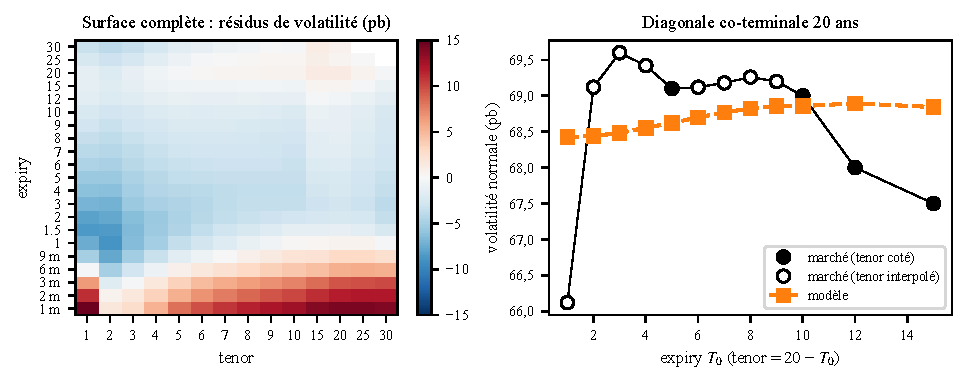
\includegraphics[width=\textwidth]{calibration_taux}
\caption{Calibration du facteur taux. À gauche, résidus du modèle calibré sur la surface complète (modèle moins
marché, en points de base de volatilité normale) ; à droite, diagonale co-terminale 20 ans, marché et modèle
calibré.}
\label{fig:calibration_taux}
\end{figure}

La vitesse de retour calibrée, 0,011, est très inférieure à l'ordre de grandeur usuel de 0,2 à 2
\citep[CM2, p.~6]{Hillairet2026}. C'est la diagonale qui l'impose ; la section~\ref{sec:resultats} montre que le
prix de l'option en dépend peu tant que cette diagonale reste reproduite.

Enfin, la diagonale permet de mesurer l'approximation à poids gelés en un facteur, où le prix exact est connu.
L'écart entre la formule de Black à poids gelés et Jamshidian ne dépasse pas 0,07~\% du prix, et une calibration
sur les prix à poids gelés donnerait $a_x = 0{,}01051$ et $\sigma_x = 0{,}7352\,\%$, des valeurs presque
identiques.

\section{Estimation du facteur spread}
\label{sec:spread}

Il n'existe pas de marché liquide d'options sur OAT d'où tirer la volatilité du spread. Il faut une autre
source d'information, et vérifier qu'elle identifie les paramètres $(a_y, \sigma_y, \rho)$. Le spread OAT–€STR
mêle crédit, liquidité et effets d'offre de titres et de collatéral (rareté des titres d'État remis en garantie,
programme d'émission du Trésor). \citet{MonfortRenne2014} identifient la liquidité par l'écart entre les titres
de la KfW, garantis par l'État fédéral allemand, et le Bund ; pour pricer une option sur OAT, seul le spread
total compte, et on ne le décompose pas.

\subsection{La courbe OAT n'identifie pas le facteur spread}
\label{sec:h1}

\citet[éq.~56-57]{Russo} calibrent le facteur spread sur la courbe des zéro-coupons risqués. Pour chaque
$\rho$ d'une grille sur $[-1,1]$, on minimise en $(a_y,\sigma_y)$ l'erreur relative entre les prix de marché
$\bar P^M(0,T_i)$ et les prix $\bar P^\ast(0,T_i) = e^{-\int_0^{T_i}\bar\alpha}$, puis on retient le $\rho$ de
plus faible erreur. Or le recalage~\eqref{eq:recalage} impose
\begin{equation}
\int_0^T\bar\alpha = -\log\bar P^M(0,T) + \tfrac12\bar V(0,T)\quad\Longrightarrow\quad
\bar P^\ast(0,T) = \bar P^M(0,T)\,e^{-\frac12\bar V(0,T)}.
\end{equation}
L'erreur à minimiser est donc $\big|e^{-\frac12\bar V(0,T)} - 1\big|$ : la procédure minimise la convexité
totale $\bar V = V_x + V_y + V_{xy}$ de la courbe OAT, et non un écart au marché. $V_x$ étant fixé par le facteur
taux, l'optimum pousse le terme croisé à compenser $V_x$, vers $\rho < 0$ et vers des $(a_y,\sigma_y)$ qui
rendent $V_y + V_{xy}$ aussi négatif que possible. La solution exacte est $\rho = -1$, $a_y = a_x$,
$\sigma_y = \sigma_x$ : le facteur spread annule alors le facteur taux ($x + y \equiv 0$), le taux OAT devient
déterministe et $\bar V \equiv 0$. Le tableau~\ref{tab:h1} le vérifie numériquement.

\begin{table}[htbp]
\centering\small
\caption{Procédure de calibration de Russo et al. appliquée à la courbe OAT ($a_x$ et $\sigma_x$ fixés)}
\label{tab:h1}
\setlength{\tabcolsep}{4pt}
\begin{tabular}{@{}lccccccccccc@{}}
\toprule
$\rho$ & $-1$ & $-0{,}8$ & $-0{,}6$ & $-0{,}4$ & $-0{,}2$ & $0$ & $0{,}2$ & $0{,}4$ & $0{,}6$ & $0{,}8$ & $1$ \\
\midrule
$a_y$ & 0,011 & 0,011 & 0,011 & 0,011 & 0,070 & 1,373 & 2,000 & 2,000 & 2,000 & 2,000 & 2,000 \\
$\sigma_y$ (\%) & 0,74 & 0,59 & 0,44 & 0,29 & 0,23 & 0,01 & 0,01 & 0,01 & 0,01 & 0,01 & 0,01 \\
Erreur (\%) & 0,000 & 2,788 & 4,860 & 6,291 & 7,136 & 7,408 & 7,409 & 7,410 & 7,411 & 7,412 & 7,414 \\
\bottomrule
\end{tabular}
\end{table}

L'erreur s'annule en $\rho = -1$ avec $(a_y, \sigma_y) = (a_x, \sigma_x)$. Pour $\rho \ge 0$, le facteur spread ne
peut qu'ajouter de la convexité : l'optimiseur ramène $\sigma_y$ sur sa borne inférieure, et l'erreur
résiduelle, 7,41~\%, est celle du seul terme de convexité du facteur taux, $|e^{-V_x/2} - 1|$. Appliquée à une courbe recalée par construction, la
procédure ne peut donc identifier aucun des trois paramètres. C'est le principe des modèles à shift
déterministe : la courbe initiale fixe le shift, et les paramètres de diffusion se calibrent sur des options
\citep[CM2, p.~30-31]{Hillairet2026}. Dans un modèle affine gaussien, la volatilité n'entre dans la coupe des
rendements que par le terme de convexité de la constante \citep[cours~3, éq.~II.8]{MPR2025}, et le recalage
absorbe ce terme. \citet[section~22.7.2]{BrigoMercurio2006} font le même constat pour l'intensité de défaut,
dont ils fixent la corrélation par estimation historique ; ils notent aussi qu'un G2++ calibré avec $\rho$
proche de $-1$ dégénère en modèle à un facteur (section~4.2.7), ce qui est l'optimum exact de la procédure.
\emph{L'hypothèse~H1 est rejetée.}

\subsection{L'information des séries historiques}

Dans le modèle, le spread de taux zéro de tenor $\tau$ vaut $c_\tau(t) + y(t)\,H_{a_y}(\tau)/\tau$, où $c_\tau$ est
déterministe. Sa volatilité instantanée est $\sigma_y H_{a_y}(\tau)/\tau$, et sa corrélation avec le taux €STR de
même tenor est $\rho$. Ce sont des propriétés des trajectoires, qui relèvent de la variation quadratique : elles
sont les mêmes sous la mesure historique et sous la mesure de pricing, car le changement de mesure de Girsanov ne
modifie que les dérives \citep[CM3, p.~5-6]{Hillairet2026}. En temps discret, un facteur d'actualisation
exponentiel-affine change de même la constante et la matrice autorégressive d'un VAR gaussien, jamais sa variance
\citep[cours~3, prop.~I.3, slides~24-25]{MPR2025}. Dans le modèle, l'égalité des volatilités sous les deux mesures
est donc un théorème ; appliquée aux données, c'est une hypothèse, celle d'une prime de risque de variance nulle,
qu'un facteur d'actualisation exponentiel-quadratique lèverait (cours~6, slides~116-117) et que l'absence d'options
sur OAT ne permet pas de tester. Le cadre de crédit va dans le même sens : quand le défaut n'est pas pricé,
l'intensité est la même fonction des facteurs sous $\P$ et sous $\Q$, et seule la dynamique des facteurs change
(cours~5, prop.~II.3).

Le coefficient $H_{a_y}(\tau)/\tau$ vient du prix d'un zéro-coupon : la vitesse de retour qui y figure est la
vitesse risque-neutre (cours~3, prop.~I.1, slide~17). La structure par terme des volatilités du spread identifie
donc $(a_y, \sigma_y)$ sous la mesure de pricing. Une volatilité décroissante avec le tenor signalerait un retour à
la moyenne ; une volatilité plate impose $a_y \approx 0$. Une régression sur le niveau du spread ne donnerait, elle,
qu'une vitesse de retour historique.

On utilise les séries quotidiennes du spread entre le rendement OAT générique et le taux de swap €STR de même
tenor, les rendements de pair servant d'approximation des taux zéro. Le tenor de deux ans est exclu : la série
générique OAT à deux ans saute de $-65$~pb le 22 janvier 2024 sans revenir, au changement du titre de référence, et
le court terme est dominé par les BTF et la politique monétaire. Le tableau~\ref{tab:vol_spread} donne les moments
par tenor sur trois fenêtres.

\begin{table}[htbp]
\centering\small
\caption{Volatilité annualisée du spread (pb par an) et corrélation de ses variations quotidiennes avec celles
du swap €STR de même tenor}
\label{tab:vol_spread}
\begin{tabular}{@{}lcccccc@{}}
\toprule
 & \multicolumn{2}{c}{2021-2026} & \multicolumn{2}{c}{Trois ans} & \multicolumn{2}{c}{Un an} \\
\cmidrule(lr){2-3}\cmidrule(lr){4-5}\cmidrule(lr){6-7}
Tenor & Volatilité & $\rho$ & Volatilité & $\rho$ & Volatilité & $\rho$ \\
\midrule
5 ans  & 33,9 & 0,064 & 28,8 & 0,067 & 26,5 & 0,272 \\
10 ans & 32,7 & 0,162 & 30,5 & 0,182 & 31,9 & 0,434 \\
15 ans & 33,2 & 0,118 & 29,8 & 0,147 & 28,2 & 0,387 \\
20 ans & 33,1 & 0,152 & 30,5 & 0,181 & 30,9 & 0,373 \\
25 ans & 33,1 & 0,148 & 30,9 & 0,169 & 30,1 & 0,360 \\
30 ans & 34,2 & 0,124 & 32,2 & 0,146 & 31,9 & 0,275 \\
\midrule
Ajustement & \multicolumn{2}{c}{$\sigma_y = 0{,}337\,\%$} & \multicolumn{2}{c}{$\sigma_y = 0{,}307\,\%$} & \multicolumn{2}{c}{$\sigma_y = 0{,}302\,\%$} \\
\bottomrule
\end{tabular}
\end{table}

La volatilité du spread est presque plate en tenor. Ajustée fenêtre par fenêtre, la structure par terme
$\sigma_y H_{a_y}(\tau)/\tau$ place $a_y$ sur sa borne inférieure de 0,001, soit une demi-vie de près de sept
siècles, dans les trois cas, avec un écart maximal de 1,0 à 3,6~pb (figure~\ref{fig:spread_historique}). La
corrélation est positive : le spread s'élargit quand les taux montent. Elle varie toutefois de 0,064 à 0,434
selon le tenor et la fenêtre, et cette fourchette servira de sensibilité.

Le modèle ne comporte qu'un facteur de spread. L'analyse en composantes principales des variations quotidiennes
du spread aux tenors 5 à 30 ans attribue 85,8~\% de leur variance à la première composante, dont les chargements
sont presque égaux d'un tenor à l'autre (de 0,36 à 0,43). Le spread se déplace surtout en bloc, ce que décrit
un facteur unique à vitesse de retour faible. La deuxième composante, une pente qui explique 8,4~\% de la variance,
reste hors du modèle.

\begin{figure}[htbp]
\centering
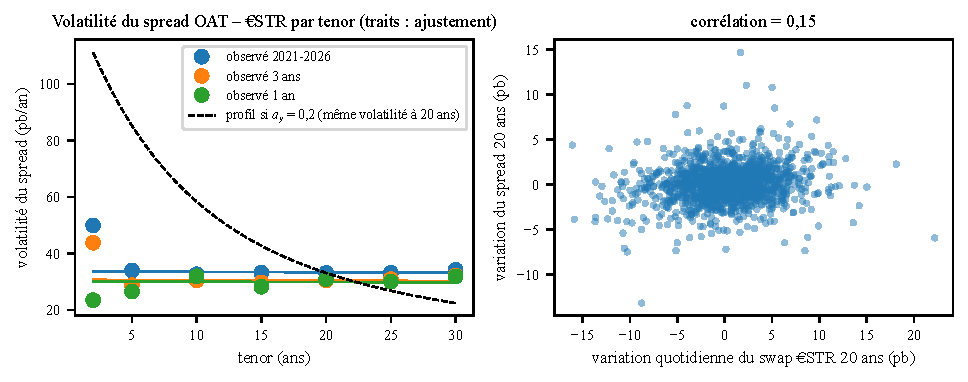
\includegraphics[width=\textwidth]{spread_historique}
\caption{À gauche, volatilité du spread OAT–€STR par tenor sur trois fenêtres (points) et structure par terme
ajustée (traits), comparée au profil qu'imposerait $a_y = 0{,}2$ ; à droite, variations quotidiennes du spread et
du swap €STR à vingt ans.}
\label{fig:spread_historique}
\end{figure}

\subsection{Estimation par la méthode des moments généralisée}

Le pricing n'a besoin que de $(a_y,\sigma_y,\rho)$, pas de toute la dynamique historique du spread : c'est le
cadre de la méthode des moments généralisée \citep[cours~5, slide~8]{Hansen1982,MPR2025}. On retient
douze moments, calculés sur 1\,451 variations quotidiennes aux dates communes des tenors 5, 10, 15, 20, 25 et
30 ans :
\begin{equation}
m^{vol}_\tau(\theta) = \sigma_y\,\frac{H_{a_y}(\tau)}{\tau},\qquad m^{corr}_\tau(\theta) = \rho,
\end{equation}
le premier pour la volatilité annualisée du spread, le second pour sa corrélation avec le swap €STR de même tenor.
Les corrélations entre spreads de tenors différents sont écartées : égales à 1 dans un modèle à un facteur,
elles le rejetteraient par construction.

Avec $\hat m$ les moments observés et $g(\theta) = m(\theta) - \hat m$, l'estimateur minimise
$g(\theta)'\,W\,g(\theta)$. La covariance $S$ des moments estimés doit tenir compte de deux propriétés des
données. Les variations quotidiennes du spread sont hétéroscédastiques : le test ARCH-LM d'\citet{Engle1982}, à
dix retards, rejette l'homoscédasticité à chaque tenor (statistique de 101 à 161, p-valeur au plus
$3{,}2\times10^{-17}$). Elles sont aussi légèrement autocorrélées. On estime donc $S$ par bootstrap par blocs
mobiles \citep{Kunsch1989}, avec des blocs de vingt jours consécutifs et 500 tirages, par le même code pour
tous les moments.

La pondération asymptotiquement efficace est $W = S^{-1}$. Mais les erreurs d'estimation des moments sont ici
très corrélées d'un tenor à l'autre, de 0,90 à 0,98 pour les volatilités et de 0,82 à 0,98 pour les corrélations
entre tenors voisins, et $S^{-1}$ combine alors les moments avec des poids implicites négatifs. L'estimation
efficace de $\rho$, 0,028, sort ainsi de l'intervalle de toutes les corrélations observées sur la période
(de 0,064 à 0,162). C'est le biais de petit échantillon de la GMM efficace appliquée aux structures de covariance,
documenté par \citet{AltonjiSegal1996}, qui recommandent une pondération diagonale. On retient donc
$W_1 = \mathrm{diag}(S)^{-1}$ : chaque moment pèse en proportion inverse de sa variance. Les écarts-types sont ceux
de la formule sandwich $(G'W_1G)^{-1}G'W_1SW_1G(G'W_1G)^{-1}$, où $G$ est la jacobienne de $g$, valide quelle que
soit la pondération. La GMM efficace sert au test de sur-identification de \citet{Hansen1982}. Comme $a_y$ bute sur
sa borne, l'inférence classique ne s'applique pas à ce paramètre : écarts-types et statistique $J$ sont calculés à
$a_y$ fixé.

\begin{table}[htbp]
\centering\small
\caption{Estimation GMM des paramètres du spread (écarts-types entre parenthèses)}
\label{tab:gmm}
\begin{tabular}{@{}lccc@{}}
\toprule
Pondération & $a_y$ & $\sigma_y$ (\%) & $\rho$ \\
\midrule
Diagonale, $W_1 = \mathrm{diag}(S)^{-1}$ (retenue) & 0,001 (borne) & 0,3374 (0,0182) & 0,130 (0,040) \\
Efficace, $W_2 = S^{-1}$ & 0,001 (borne) & 0,3257 (0,0141) & 0,028 (0,034) \\
\midrule
\multicolumn{4}{@{}l}{Test de Hansen : $J = 73{,}7$ pour 10 degrés de liberté, p-valeur $8{,}7\times10^{-12}$} \\
\bottomrule
\end{tabular}
\end{table}

L'estimation retenue (tableau~\ref{tab:gmm}) donne une volatilité du spread de 33,7~pb par an et une corrélation de
0,13, la vitesse de retour restant sur sa borne. Les volatilités ajustées vont de 33,2 à 33,7~pb selon le tenor,
pour des volatilités observées de 32,7 à 34,2~pb. Le test $J$ rejette le modèle. Avec près de 1\,450 observations,
le test est très puissant : il rejette un spread à un facteur qui ne reproduit ni des corrélations variant d'un
tenor à l'autre, ni la légère hausse des volatilités aux tenors extrêmes. Les estimations se lisent alors comme les
paramètres du modèle à un facteur le plus proche des moments observés. Les paramètres retenus pour la suite sont
\begin{equation}
a_x = 0{,}0107,\quad \sigma_x = 0{,}7367\,\%,\qquad a_y = 0{,}001,\quad \sigma_y = 0{,}3374\,\%,\quad \rho = 0{,}130.
\end{equation}

\subsection{Régimes de volatilité du spread}
\label{sec:regimes}

La méthode des moments suppose la volatilité du spread constante, alors que le test ARCH-LM rejette
l'homoscédasticité : $\sigma_y$ est une moyenne sur la période. Pour les spreads souverains de la zone euro,
\citet{MonfortRenne2014} emploient un modèle à deux régimes, dont un régime de crise
\citep[cours~5, slides~99-101]{MPR2025}. On ajuste le modèle de régression à changement de régime du cours
(slides~25 et~29) à la variation quotidienne du spread à vingt ans, expliquée par celle du swap €STR de même
tenor :
\begin{equation}
\Delta S_t = c_{k_t} + \beta_{k_t}\,\Delta R_t + \sigma_{k_t}\,\varepsilon_t,\qquad \varepsilon_t \sim \mathcal N(0,1)\ \text{i.i.d.},
\end{equation}
où le régime $k_t$, calme ou agité, suit une chaîne de Markov à deux états non observée. Le filtre de
Kitagawa-Hamilton donne la vraisemblance, maximisée en $(c_k, \beta_k, \sigma_k)$ et en les probabilités de
transition \citep[cours~5, slide~39]{Hamilton1989,MPR2025} ; l'algorithme de \citet{Kim1994} donne les
probabilités lissées des régimes. Dans chaque régime, la volatilité du spread et sa corrélation avec le swap se
calculent sur les variations pondérées par ces probabilités, et la part du temps passée dans chaque régime est sa
probabilité stationnaire (cours~5, slide~35).

\begin{table}[htbp]
\centering\small
\caption{Régimes de volatilité du spread à vingt ans (durées en jours ouvrés, volatilités en pb par an)}
\label{tab:regimes}
\begin{tabular}{@{}llccccc@{}}
\toprule
Variations & Régime & Part du temps & Durée moyenne & Vol. du spread & Vol. du swap & $\rho$ \\
\midrule
\multirow{2}{*}{Quotidiennes} & calme & 0,73 & 43 & 23,0 & 59,7 & 0,16 \\
 & agité & 0,27 & 16 & 51,1 & 89,4 & 0,15 \\
\midrule
\multirow{2}{*}{Hebdomadaires} & calme & 0,65 & 137 & 19,0 & 57,8 & 0,22 \\
 & agité & 0,35 & 73 & 42,6 & 95,2 & $-0{,}01$ \\
\bottomrule
\end{tabular}
\end{table}

Deux régimes se dégagent nettement (tableau~\ref{tab:regimes}). Sur variations quotidiennes, le régime calme
occupe 73~\% du temps, avec une volatilité du spread de 23~pb par an, et le régime agité 27~\%, avec 51~pb. Les
épisodes agités coïncident avec la remontée des taux de 2022 et du début de 2023, puis avec les crises politiques
françaises de juin 2024 (dissolution de l'Assemblée nationale) et de l'automne 2024 (budget, censure du
gouvernement) ; la figure~\ref{fig:regimes} les situe. Au 8 septembre 2026, la probabilité filtrée du régime
agité est de 8~\%.

\begin{figure}[htbp]
\centering
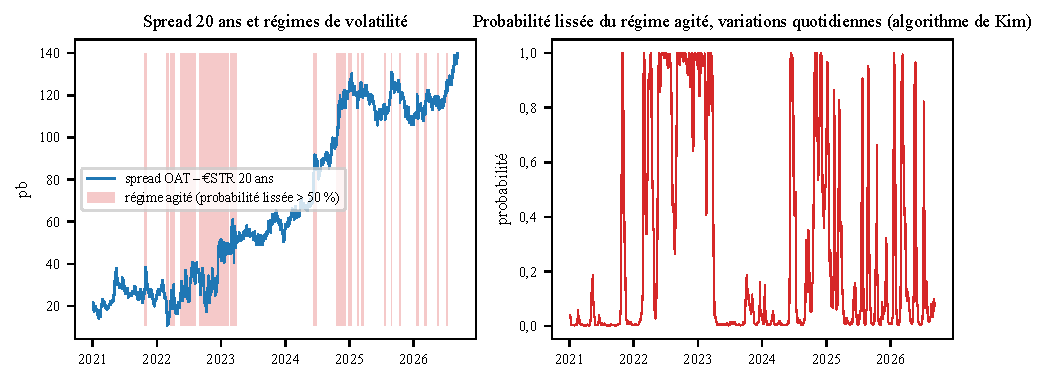
\includegraphics[width=\textwidth]{regimes}
\caption{Spread OAT–€STR à vingt ans et probabilité lissée du régime agité (variations quotidiennes).}
\label{fig:regimes}
\end{figure}

Deux résultats comptent pour la suite. La corrélation n'est pas liée aux régimes : presque la même dans les deux
régimes sur variations quotidiennes (0,16 et 0,15), elle s'annule dans le régime agité sur variations
hebdomadaires. Les régimes de volatilité n'expliquent donc pas la fourchette de $\rho$ selon les fenêtres. Les
régimes sont par ailleurs courts au regard des échéances d'options : 43 et 16 jours ouvrés en moyenne sur variations
quotidiennes, 137 et 73 sur variations hebdomadaires. La section~\ref{sec:resultats} en mesure l'effet sur le prix.

\section{Estimation par filtre de Kalman}
\label{sec:kalman}

La méthode des moments n'utilise que les variations quotidiennes du spread. Elle ignore la dynamique de son
niveau, donc la mesure historique, et traite chaque série comme une observation exacte du facteur. Or le facteur
$y$ n'est pas observé : seuls le sont des rendements de différentes maturités, qui en dépendent avec une erreur.
Le cadre naturel est alors celui des modèles espace-état, estimés par maximum de vraisemblance à l'aide du filtre
de Kalman \citep[cours~5, section~I.2]{MPR2025}. Le filtre estime ensemble les paramètres risque-neutres, qui
fixent les chargements des rendements sur les facteurs, et les paramètres historiques, qui fixent la dynamique
des facteurs ; il reconstruit aussi la trajectoire des facteurs. On l'emploie ici en contrôle de la GMM, et pour
tester ce que les données disent de la mesure historique.

\subsection{Représentation espace-état}

On observe chaque jour ouvré $t$ les taux de swaps €STR $R_t(\tau)$ et les spreads OAT–€STR $S_t(\tau)$ aux six
tenors $\tau \in \{5, 10, 15, 20, 25, 30\}$ ans, soit un vecteur $z_t$ de $m = 12$ séries, centrées sur leur moyenne
empirique. L'état est le couple non observé $w_t = (x_t, y_t)'$. Dans le modèle, le taux zéro €STR de maturité
$\tau$ est affine en $x$, de pente $H_{a_x^Q}(\tau)/\tau$, et le spread zéro est affine en $y$, de pente
$H_{a_y^Q}(\tau)/\tau$. D'où l'équation de mesure (cours~5, définition~I.1)
\begin{equation}
z_t = B\,w_t + \varepsilon_t,\qquad
B = \begin{pmatrix} \big(H_{a_x^Q}(\tau_j)/\tau_j\big)_j & 0 \\ 0 & \big(H_{a_y^Q}(\tau_j)/\tau_j\big)_j \end{pmatrix},
\end{equation}
avec $\varepsilon_t \sim \mathcal N(0,\Omega)$ et $\Omega = \mathrm{diag}(\omega_1^2, \dots, \omega_{12}^2)$,
où les chargements dépendent des vitesses de retour risque-neutres $a^Q$, celles qui figurent dans les prix des
zéro-coupons. Sous la mesure historique, les facteurs suivent des processus d'Ornstein-Uhlenbeck de vitesses
$a^P$, avec les mêmes volatilités et la même corrélation ; les dynamiques sous les deux mesures sont spécifiées
séparément, comme dans la modélisation mixte du cours~1 (slide~132). Discrétisés exactement au pas
$\Delta = 1/252$, ils donnent l'équation de transition, un VAR(1) gaussien :
\begin{equation}
\begin{split}
w_t &= \Phi\,w_{t-1} + \eta_t,\qquad \Phi = \mathrm{diag}\big(e^{-a_x^P\Delta},\,e^{-a_y^P\Delta}\big),\\
\Var(\eta_t) &= \begin{pmatrix} \sigma_x^2\,I(2a_x^P) & \rho\sigma_x\sigma_y\,I(a_x^P + a_y^P) \\
\rho\sigma_x\sigma_y\,I(a_x^P + a_y^P) & \sigma_y^2\,I(2a_y^P)\end{pmatrix},
\end{split}
\end{equation}
avec $I(a) = (1-e^{-a\Delta})/a$. Les paramètres sont
$\theta = (a_x^Q, a_y^Q, a_x^P, a_y^P, \sigma_x, \sigma_y, \rho, \omega_1, \dots, \omega_{12})$.

C'est la représentation espace-état de Diebold, Rudebusch et Aruoba \citep[cours~3, slides~119-120]{MPR2025},
avec des chargements contraints par l'absence d'arbitrage : $H_a(\tau)/\tau$ est le chargement de pente de
Nelson-Siegel, qui tend vers le chargement de niveau, égal à 1, quand $a \to 0$. Une vitesse risque-neutre nulle
fait donc du facteur un facteur de niveau.

\subsection{Vraisemblance et identification}

Le modèle est linéaire et gaussien : le filtre de Kalman donne exactement la loi de $w_t$ sachant les observations
passées (cours~5, proposition~I.2), et la vraisemblance se calcule à partir des erreurs de prévision
$\nu_t = z_t - B\,w_{t|t-1}$ et de leurs variances $S_t$ :
\begin{equation}
\log L(\theta) = -\frac{mT}{2}\log 2\pi - \frac12\sum_{t=1}^T\Big(\log|S_t| + \nu_t'\,S_t^{-1}\,\nu_t\Big).
\end{equation}
Le filtre est initialisé à la loi stationnaire de l'état, et les quelques valeurs manquantes des séries €STR sont
traitées en réduisant ces jours-là la dimension de $z_t$ (cours~5, remarques~I.2 et~I.3). La vraisemblance est
maximisée par l'algorithme L-BFGS ; le filtre, la vraisemblance et le lissage sont ceux de la classe
\texttt{MLEModel} de statsmodels.

Laissée libre, la vraisemblance est maximale lorsque l'une des variances d'erreur s'annule : le facteur passe alors
exactement par une série, et la vraisemblance a plusieurs maxima selon la série choisie. On fixe ce choix en
supposant les deux taux à vingt ans, tenor de l'OAT sous-jacente, observés sans erreur. C'est l'hypothèse des
variables parfaitement modélisées de la technique d'inversion de \citet{ChenScott1993}
(cours~5, section~I.3, hypothèse~I.1) : les facteurs se lisent sur les taux à vingt ans, et les dix autres séries,
mesurées avec erreur, identifient les vitesses risque-neutres par la forme de leurs chargements.

\subsection{Ce que le filtre peut identifier : test sur données simulées}

Avant l'estimation sur données réelles, on vérifie ce que l'estimateur retrouve quand le modèle est vrai. On simule
48 échantillons de 1\,460 jours, la taille des données, aux paramètres estimés plus bas, à trois exceptions près :
$a_y^Q = 0{,}05$, pour savoir si une vitesse risque-neutre modeste serait détectée, et $a_x^P = a_y^P = 0{,}2$,
ordre de grandeur courant d'une vitesse historique (demi-vie de 3,5 ans). Le modèle est réestimé sur chaque
échantillon.

\begin{table}[htbp]
\centering\small
\caption{Estimation sur 48 échantillons simulés (volatilités en \%)}
\label{tab:kalman_sim}
\begin{tabular}{@{}lccccc@{}}
\toprule
 & Valeur vraie & Médiane & Écart-type & Quantile 5~\% & Quantile 95~\% \\
\midrule
$a_x^Q$ & 0,0118 & 0,0117 & 0,0006 & 0,0109 & 0,0126 \\
$a_y^Q$ & 0,0500 & 0,0499 & 0,0015 & 0,0480 & 0,0526 \\
$a_x^P$ & 0,2000 & 0,8173 & 0,6231 & 0,2291 & 2,3023 \\
$a_y^P$ & 0,2000 & 0,6166 & 0,7056 & 0,1042 & 1,7754 \\
$\sigma_x$ & 0,7751 & 0,7734 & 0,0163 & 0,7439 & 0,7970 \\
$\sigma_y$ & 0,3313 & 0,3301 & 0,0081 & 0,3183 & 0,3420 \\
$\rho$ & 0,1513 & 0,1511 & 0,0253 & 0,1147 & 0,1930 \\
\bottomrule
\end{tabular}
\end{table}

Les paramètres qui fixent les chargements et les covariances sont retrouvés avec précision
(tableau~\ref{tab:kalman_sim}) : une vitesse risque-neutre de 0,05 serait détectée sans ambiguïté. Les vitesses
historiques ne le sont pas. Sur six ans de données, un processus de demi-vie 3,5 ans ne parcourt qu'environ un
cycle, et la vraisemblance distingue mal une vitesse de 0,2 d'une vitesse de 1. L'estimateur est de plus biaisé :
en petit échantillon, le coefficient autorégressif $\phi = e^{-a^P\Delta}$ d'un processus persistant est
sous-estimé d'environ $(1+3\phi)/T$ (approximation de Kendall, cours~5, slides~52-53), donc la vitesse
$a^P \approx (1-\phi)/\Delta$ est surestimée d'environ $4/(T\Delta)$, soit 0,7 pour $T\Delta \approx 5{,}8$ années.
C'est l'ordre de grandeur de l'écart entre les médianes estimées, 0,82 et 0,62, et la vraie valeur. On retrouve le
problème de persistance du cours (section~I.6).

\subsection{Résultats sur données françaises}

\begin{table}[htbp]
\centering\small
\caption{Estimation par filtre de Kalman, 1\,460 jours du 4 janvier 2021 au 8 septembre 2026 (volatilités en \%)}
\label{tab:kalman}
\begin{tabular}{@{}lccc@{}}
\toprule
 & Filtre de Kalman & Écart-type & GMM ou swaptions \\
\midrule
$a_x^Q$ & 0,0118 & 0,0004 & 0,0107 \\
$a_y^Q$ & 0,0001 & 0,0004 & 0,001 (borne) \\
$a_x^P$ & 0,1216 & 0,1587 & — \\
$a_y^P$ & 0,2152 & 0,3591 & — \\
$\sigma_x$ & 0,7751 & 0,0123 & 0,7367 \\
$\sigma_y$ & 0,3313 & 0,0038 & 0,3374 \\
$\rho$ & 0,1513 & 0,0211 & 0,1299 \\
\bottomrule
\end{tabular}
\end{table}

Les estimations confirment la mesure de pricing (tableau~\ref{tab:kalman}). La vitesse risque-neutre du spread est
nulle, comme dans la GMM ; la volatilité du spread, 33,1~pb par an, et sa corrélation avec les taux, 0,15, sont
proches de celles de la GMM. La vitesse risque-neutre des taux, tirée de la seule coupe de la courbe €STR, vaut
0,0118, proche de celle qu'impliquent les swaptions (0,0107). Les vitesses historiques ne sont pas significatives,
ce que le test sur données simulées laissait prévoir.

Les écarts-types des erreurs de mesure vont de 5 à 27~pb pour les swaps €STR et de 4 à 12~pb pour les spreads,
les plus élevés au tenor de cinq ans. Le test de \citet{LjungBox1978}, à dix retards, rejette l'indépendance des
erreurs de prévision pour chaque série (p-valeur au plus $2{,}9\times10^{-261}$) : les écarts de chaque tenor au
facteur sont persistants. Un facteur par courbe ne reproduit pas les déformations de pente, que la deuxième
composante principale du spread mettait déjà en évidence ; la figure~\ref{fig:kalman} le montre au tenor de cinq
ans. C'est la conclusion du test $J$ de la GMM.

\begin{figure}[htbp]
\centering
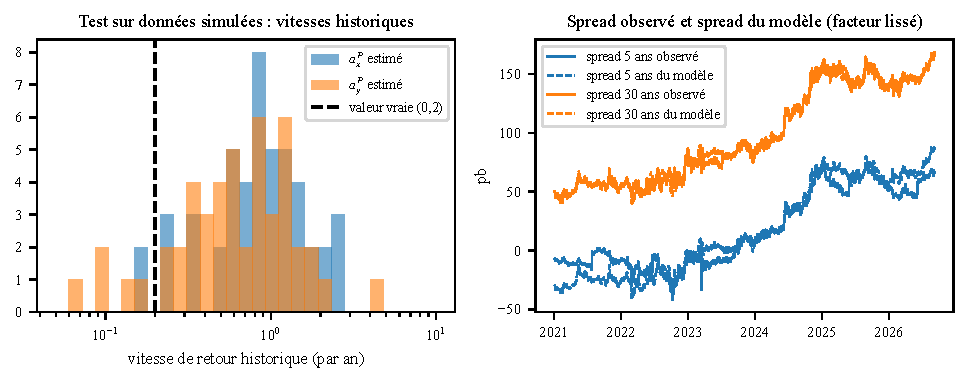
\includegraphics[width=\textwidth]{kalman}
\caption{À gauche, vitesses historiques estimées sur les 48 échantillons simulés (valeur vraie 0,2) ; à droite,
spreads observés et spreads du modèle à 5 et 30 ans, avec le facteur lissé.}
\label{fig:kalman}
\end{figure}

Le filtre de Kalman confirme ainsi l'hypothèse~H2 pour la mesure de pricing et la rejette pour la mesure
historique. La volatilité, la corrélation et la vitesse risque-neutre du spread sont identifiées et concordent
avec la GMM ; six ans de données ne suffisent pas, en revanche, à identifier sa dynamique historique. La GMM reste
l'estimateur retenu, et la section~\ref{sec:resultats} mesure l'effet sur le prix d'un passage aux paramètres du
filtre.

\section{Validation et résultats}
\label{sec:resultats}

Les résultats portent sur l'OAT 4,10~\% 2046, pour des options d'échéance 1, 2, 5, 7 et 10 ans et des strikes
clean de 90 à 110~\% du forward clean, avec les paramètres retenus aux sections~\ref{sec:taux}
et~\ref{sec:spread}. On valide d'abord le prix exact, puis on reprend les hypothèses H5, H3 et H4.

\subsection{Validation du prix exact et précision des poids gelés}

Le prix~\eqref{eq:prix_exact} est exact au calcul de l'intégrale près. On le valide par un Monte-Carlo
indépendant. Le prix s'écrit
$\E^{\Q}\big[e^{-\int_0^{T_0}r}\,(\bar B(T_0)-X)^+\big]$, et tout ce qui y entre est fonction du vecteur
gaussien $Z = \big(x(T_0), y(T_0), \int_0^{T_0}x, \int_0^{T_0}y\big)$, de moyenne nulle sous $\Q$ et de covariance
donnée en annexe~A. On simule $Z$ exactement, sans discrétisation en temps : le facteur d'actualisation vaut
$P^M(0,T_0)\,e^{-\frac12V_x(0,T_0)}\,e^{-\int_0^{T_0}x}$, et $\bar B(T_0)$ s'obtient par la formule
fermée~\eqref{eq:zc_oat}, le facteur spread étant décalé du recentrage $\delta$. La simulation utilise 400\,000
trajectoires avec variables antithétiques.

Trois contrôles précèdent le pricing, à cinq ans. La moyenne simulée de $e^{-\int r}$ vaut 0,863309, pour
$P^M(0,5) = 0{,}863309$. Celle de $e^{-\int \bar r}$ vaut 0,839610, pour $\bar P^M(0,5) = 0{,}839609$, ce qui
teste le recalage de la courbe OAT et toute la matrice de covariance. Enfin, le forward simulé vaut 87,903, pour
un forward repo de 87,908 : la loi forward et le recentrage sont corrects. Dans le cas limite à un facteur
($\sigma_y = 0$, courbe OAT confondue avec la courbe €STR), le prix exact du call à la monnaie à cinq ans,
6,254832, est égal à celui de Jamshidian à la sixième décimale.

\begin{table}[htbp]
\centering\small
\caption{Prix exact, Monte-Carlo (MC, demi-largeur de l'intervalle de confiance à 95~\%) et approximation à poids
gelés, $T_0 = 5$ ans (prix pour 100 de nominal ; écarts relatifs en \%)}
\label{tab:validation}
\begin{tabular}{@{}llcccccc@{}}
\toprule
Strike & Type & Exact & MC & IC 95~\% & Exact/MC $-1$ & Poids gelés & Gelés/exact $-1$ \\
\midrule
90~\%  & call & 9,9609 & 9,9513 & 0,0249 & 0,10 & 10,0170 & 0,56 \\
90~\%  & put  & 2,4752 & 2,4696 & 0,0118 & 0,23 & 2,5313 & 2,27 \\
100~\% & call & 5,7627 & 5,7512 & 0,0259 & 0,20 & 5,7695 & 0,12 \\
100~\% & put  & 5,7627 & 5,7552 & 0,0131 & 0,13 & 5,7695 & 0,12 \\
110~\% & call & 3,0727 & 3,0661 & 0,0217 & 0,22 & 3,0292 & $-1{,}42$ \\
110~\% & put  & 10,5584 & 10,5558 & 0,0085 & 0,02 & 10,5149 & $-0{,}41$ \\
\bottomrule
\end{tabular}
\end{table}

Le prix exact reste dans l'intervalle de confiance du Monte-Carlo pour tous les strikes
(tableau~\ref{tab:validation}) et, à la monnaie, à toutes les échéances, où la demi-largeur relative de
l'intervalle va de 0,4 à 0,5~\%. Le prix exact sert donc de référence pour mesurer l'erreur de l'approximation à
poids gelés, sans bruit de simulation.

\begin{table}[htbp]
\centering\small
\caption{Erreur relative de l'approximation à poids gelés (poids forward recentrés) contre le prix exact, en \%}
\label{tab:poids_geles}
\begin{tabular}{@{}lccccc@{}}
\toprule
 & 1 an & 2 ans & 5 ans & 7 ans & 10 ans \\
\midrule
Call 90~\%  & 0,29 & 0,46 & 0,56 & 0,52 & 0,38 \\
Call 100~\% & 0,04 & 0,08 & 0,12 & 0,11 & 0,08 \\
Call 110~\% & $-2{,}98$ & $-2{,}18$ & $-1{,}42$ & $-1{,}17$ & $-0{,}92$ \\
Put 90~\%   & 4,28 & 3,22 & 2,27 & 1,91 & 1,45 \\
Put 110~\%  & $-0{,}28$ & $-0{,}39$ & $-0{,}41$ & $-0{,}37$ & $-0{,}28$ \\
\midrule
\multicolumn{6}{@{}l}{\footnotesize Poids gelés à leur valeur d'aujourd'hui, call 100~\% : de $-0{,}04$ à $+0{,}50$ (à 10 ans)} \\
\bottomrule
\end{tabular}
\end{table}

À la monnaie, l'approximation de \citet{Russo} s'écarte du prix exact de 0,12~\% au plus lorsque les poids sont
gelés à leur valeur forward recentrée, contre 0,5~\% à dix ans s'ils sont gelés à leur valeur d'aujourd'hui
(tableau~\ref{tab:poids_geles}). En dehors de la monnaie, l'erreur grandit quand l'échéance raccourcit : de
$-0{,}9\,\%$ à dix ans à $-3{,}0\,\%$ à un an sur le call à 110~\%, de $+1{,}4\,\%$ à $+4{,}3\,\%$ sur le put à
90~\%. La loi du prix de l'OAT, somme de lognormales, n'est pas lognormale : l'approximation sous-évalue sa queue
droite et surévalue sa queue gauche, et l'erreur relative pèse d'autant plus que l'option est loin de la monnaie
en nombre d'écarts-types, donc que l'échéance est courte (figure~\ref{fig:validation}).
\emph{L'hypothèse~H5 est confirmée à la monnaie et rejetée en dehors} ; le pricer utilise le prix exact.

\begin{figure}[htbp]
\centering
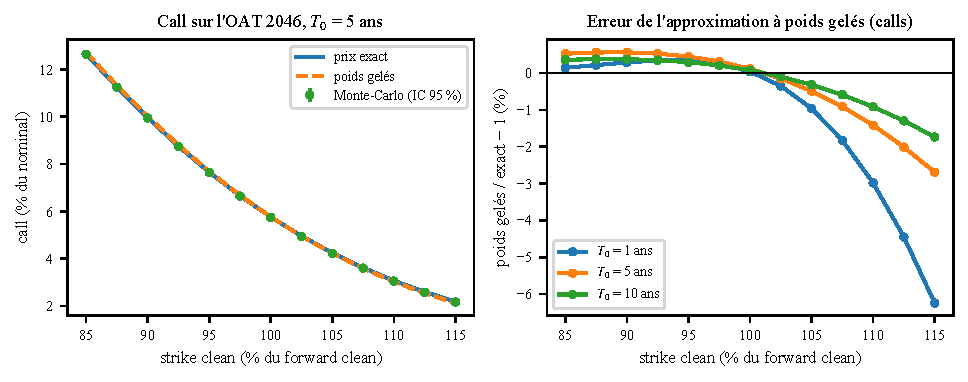
\includegraphics[width=\textwidth]{validation}
\caption{À gauche, call à cinq ans selon le strike : prix exact, poids gelés et Monte-Carlo ; à droite, erreur
relative des poids gelés selon le strike, à 1, 5 et 10 ans.}
\label{fig:validation}
\end{figure}

\subsection{Effet du facteur spread}
\label{sec:h3}

On compare le modèle à deux facteurs calibré au facteur taux seul ($\sigma_y = 0$, même forward repo, même
courbe), c'est-à-dire à ce que donnerait un pricer Hull-White calibré sur les seules swaptions €STR.

\begin{table}[htbp]
\centering\small
\caption{Effet du facteur spread sur le call à la monnaie forward (prix pour 100 de nominal)}
\label{tab:h3}
\begin{tabular}{@{}lccccccccc@{}}
\toprule
 & & \multicolumn{2}{c}{$\bar\Sigma_B$} & \multicolumn{3}{c}{Parts de $\bar\Sigma_B^2$} & \multicolumn{3}{c}{Call à la monnaie} \\
\cmidrule(lr){3-4}\cmidrule(lr){5-7}\cmidrule(lr){8-10}
$T_0$ & $F^{clean}$ & 2F & Taux seul & Taux & Spread & Croisée & 2F & Taux seul & Écart \\
\midrule
1 an   & 90,363 & 0,1007 & 0,0859 & 0,727 & 0,179 & 0,094 & 3,5781 & 3,0512 & +17,3~\% \\
2 ans  & 89,323 & 0,1373 & 0,1170 & 0,726 & 0,180 & 0,094 & 4,6770 & 3,9878 & +17,3~\% \\
5 ans  & 86,709 & 0,1909 & 0,1625 & 0,725 & 0,181 & 0,094 & 5,7627 & 4,9109 & +17,3~\% \\
7 ans  & 85,618 & 0,2030 & 0,1727 & 0,724 & 0,181 & 0,094 & 5,6794 & 4,8378 & +17,4~\% \\
10 ans & 85,266 & 0,1971 & 0,1677 & 0,724 & 0,182 & 0,094 & 4,9598 & 4,2223 & +17,5~\% \\
\bottomrule
\end{tabular}
\end{table}

Avec les paramètres estimés, le spread apporte 18~\% de la variance du prix forward de l'OAT, et le terme croisé
9~\% de plus, car $\rho > 0$ : le spread s'élargit quand les taux montent (tableau~\ref{tab:h3}). La volatilité
$\bar\Sigma_B$ dépasse de 17 à 18~\% celle du facteur taux seul, et le call à la monnaie est plus cher de 17~\% à
toutes les échéances (figure~\ref{fig:resultats}). \emph{L'hypothèse~H3 est confirmée.}

Le call à la monnaie croît jusqu'à cinq ans, puis décroît. Au-delà de cinq ans, l'obligation restante raccourcit :
sa volatilité de prix plafonne vers sept ans puis baisse, et le forward comme l'actualisation diminuent. Le forward
clean passe de 90,4 à un an à 85,3 à dix ans : porter une OAT qui rapporte plus que son financement fait baisser
son prix forward, et l'effet s'accumule avec l'échéance. Le recentrage $\delta$ vaut $-2{,}6$, $-3{,}2$, $-0{,}9$,
$8{,}3$ et $33{,}0$~pb aux cinq échéances : la courbe repo retenue est du même ordre que le spread de l'OAT, un peu
au-dessus à un an et en dessous à dix ans, et l'approximation que porte $\delta$ (section~\ref{sec:evaluation})
reste limitée.

\begin{figure}[htbp]
\centering
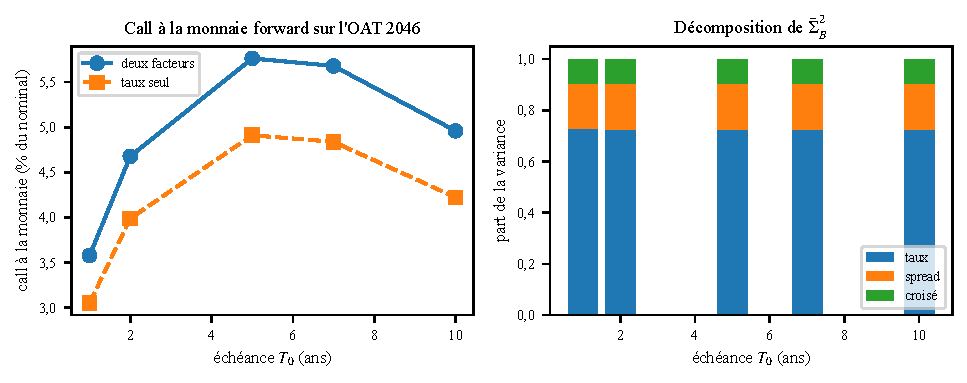
\includegraphics[width=\textwidth]{resultats}
\caption{À gauche, call à la monnaie forward selon l'échéance, modèle à deux facteurs et facteur taux seul ; à
droite, décomposition de $\bar\Sigma_B^2$ en parts taux, spread et croisée.}
\label{fig:resultats}
\end{figure}

\subsection{Un facteur suffit-il ?}
\label{sec:h4}

La répartition de la variance ne dépend presque pas de l'échéance, parce que les deux vitesses de retour sont
faibles : $H_{a_x} \approx H_{a_y}$, les deux facteurs déplacent les prix de la même façon, et leur somme se
comporte comme un facteur unique de volatilité
$\sigma_{eq} = \sqrt{\sigma_x^2 + \sigma_y^2 + 2\rho\sigma_x\sigma_y} = 0{,}849\,\%$, contre $\sigma_x = 0{,}737\,\%$.
On le vérifie avec un Hull-White à un facteur sur la courbe OAT, de vitesse $a_x$ et de volatilité $\sigma_{eq}$.

\begin{table}[htbp]
\centering\small
\caption{Hull-White à un facteur équivalent contre modèle à deux facteurs}
\label{tab:h4}
\begin{tabular}{@{}lccccc@{}}
\toprule
 & \multicolumn{3}{c}{Volatilité $\sigma_{eq} = 0{,}849\,\%$} & \multicolumn{2}{c}{Volatilité ajustée à la monnaie} \\
\cmidrule(lr){2-4}\cmidrule(lr){5-6}
$T_0$ & Call 2F & Call 1F & Écart à la monnaie & Volatilité (\%) & Écart max. 90-110~\% \\
\midrule
1 an   & 3,5781 & 3,5165 & $-1{,}72$~\% & 0,8641 & 0,053~\% \\
2 ans  & 4,6770 & 4,5951 & $-1{,}75$~\% & 0,8644 & 0,037~\% \\
5 ans  & 5,7627 & 5,6572 & $-1{,}83$~\% & 0,8651 & 0,020~\% \\
7 ans  & 5,6794 & 5,5729 & $-1{,}87$~\% & 0,8655 & 0,014~\% \\
10 ans & 4,9598 & 4,8643 & $-1{,}92$~\% & 0,8659 & 0,008~\% \\
\bottomrule
\end{tabular}
\end{table}

Le Hull-White à un facteur reproduit le call à la monnaie du modèle à deux facteurs à 1,9~\% près à toutes les
échéances, un peu en dessous, la sensibilité $H_{a_y}$ au spread dépassant légèrement $H_{a_x}$
(tableau~\ref{tab:h4}). En dehors de la monnaie, l'écart grandit jusqu'à $-5{,}1\,\%$ sur le put à 90~\% à un an,
mais il ne tient qu'au niveau de $\sigma_{eq}$, un peu trop bas. Avec une volatilité ajustée sur le call à la
monnaie, de 0,864 à 0,866~\%, le modèle à un facteur reproduit les prix du modèle à deux facteurs de 90 à 110~\% du
forward à 0,05~\% près. Le second facteur ne change donc pas la forme de la loi du prix de l'OAT à l'échéance,
seulement sa dispersion. Pour une option sur une seule OAT, il agit comme un supplément de volatilité ; sa
structure propre ne compterait que pour des produits sensibles à l'écart entre les deux courbes, comme les options
sur spread ou sur plusieurs titres. C'est la frontière que tracent \citet[section~4.1]{BrigoMercurio2006} entre
modèles à un et à deux facteurs, et \citet[section~6.4.6]{Chaix2021} de même : un facteur suffit quand les taux qui
font le payoff sont presque parfaitement corrélés. Avec des vitesses quasi nulles, chaque facteur est proche d'un
modèle de Ho et Lee, limite du Vasicek quand $a \to 0$ \citep[CM3, p.~14]{Hillairet2026}, et leur somme aussi.
\emph{L'hypothèse~H4 est rejetée avec les paramètres estimés.}

\subsection{Cohérence de la calibration mixte}

Le facteur taux est calibré sur des volatilités implicites, le facteur spread sur des volatilités historiques. Le
modèle calibré donne au swap €STR à vingt ans une volatilité de 66,3~pb par an et au rendement OAT à vingt ans
78,1~pb ; sur 2021-2026, les volatilités réalisées sont de 69,1 et 81,0~pb. Le rapport OAT~/~€STR, qui mesure
l'effet du spread, vaut 1,177 dans le modèle et 1,173 dans les données. Le contrôle n'est pas indépendant de la
calibration, puisque la volatilité du spread et $\rho$ viennent des mêmes séries, mais il montre que la volatilité
implicite des swaptions et les volatilités historiques ne se contredisent pas sur la période.

Comme un facteur d'actualisation exponentiel-affine laisse la variance inchangée, ce contrôle teste, pour les taux,
l'absence de prime de risque de variance que l'on doit supposer pour le spread. Le filtre de Kalman, estimé sur les
seules séries, permet de mener ce test sur toute la diagonale : avec sa volatilité historique des taux (0,775~\%),
il surévalue les volatilités des swaptions de 2,8~pb en moyenne (de 1,7 à 5,2~pb). La volatilité implicite à la
même vitesse de retour est de 0,744~\%, et le rapport $\sigma^{\Q}/\sigma^{\P}$ vaut 0,96. L'écart est
significatif, à 2,5 écarts-types, mais faible : s'il valait aussi pour le spread, il ne réduirait le call à la
monnaie que de 0,9~\%.

\subsection{Sensibilités}

Le tableau~\ref{tab:sensibilites} rassemble les variations du call à la monnaie dans chaque scénario, par rapport
au cas central.

\begin{table}[htbp]
\centering\small
\caption{Variation du call à la monnaie par rapport au cas central, en \%}
\label{tab:sensibilites}
\begin{tabular}{@{}llrrrrr@{}}
\toprule
Paramètre & Scénario & 1 an & 2 ans & 5 ans & 7 ans & 10 ans \\
\midrule
\multirow{2}{*}{Volatilité du spread} & $\sigma_y$ divisée par 2 & $-9{,}5$ & $-9{,}5$ & $-9{,}5$ & $-9{,}6$ & $-9{,}6$ \\
 & $\sigma_y$ multipliée par 2 & $+27{,}7$ & $+27{,}7$ & $+27{,}7$ & $+27{,}8$ & $+27{,}9$ \\
\multirow{2}{*}{Corrélation} & $\rho = 0{,}064$ & $-2{,}4$ & $-2{,}4$ & $-2{,}4$ & $-2{,}4$ & $-2{,}4$ \\
 & $\rho = 0{,}434$ & $+10{,}4$ & $+10{,}4$ & $+10{,}4$ & $+10{,}4$ & $+10{,}4$ \\
\multirow{2}{*}{Vitesse du spread} & $a_y = 0{,}215$ & $+4{,}3$ & $+2{,}6$ & $-0{,}7$ & $-1{,}7$ & $-1{,}9$ \\
 & $a_y = 1$ & $-0{,}3$ & $-5{,}2$ & $-9{,}6$ & $-10{,}3$ & $-10{,}2$ \\
Estimation du spread & filtre de Kalman & $+0{,}5$ & $+0{,}5$ & $+0{,}5$ & $+0{,}5$ & $+0{,}5$ \\
\multirow{2}{*}{Vitesse des taux} & $a_x = 0{,}05$ & $+2{,}9$ & $+2{,}3$ & $+0{,}8$ & $+0{,}1$ & $-0{,}4$ \\
 & $a_x = 0{,}2$ & $+14{,}9$ & $+9{,}8$ & $-0{,}1$ & $-3{,}0$ & $-3{,}2$ \\
\multirow{3}{*}{Régimes} & toujours calme & $-5{,}9$ & $-5{,}9$ & $-5{,}9$ & $-6{,}0$ & $-6{,}0$ \\
 & toujours agité & $+14{,}6$ & $+14{,}6$ & $+14{,}6$ & $+14{,}6$ & $+14{,}7$ \\
 & régimes simulés (hebdomadaires) & $-0{,}6$ & $-0{,}3$ & $-0{,}1$ & $-0{,}1$ & $-0{,}1$ \\
\multirow{3}{*}{Spread repo (fictif)} & courbe $-25$~pb & $-3{,}3$ & $-5{,}1$ & $-9{,}8$ & $-13{,}5$ & $-20{,}7$ \\
 & courbe $+25$~pb & $+3{,}4$ & $+5{,}2$ & $+10{,}5$ & $+14{,}8$ & $+23{,}9$ \\
 & financement au taux de l'OAT & $-0{,}6$ & $-0{,}6$ & $+3{,}1$ & $+10{,}6$ & $+27{,}1$ \\
\bottomrule
\end{tabular}
\end{table}

La corrélation est le paramètre le moins bien connu : sa fourchette historique, de 0,06 à 0,43, est bien plus
large que l'incertitude statistique de l'estimation, et le call y varie de $-2\,\%$ à $+10\,\%$. La vitesse de
retour du spread, à volatilité du spread à vingt ans inchangée puisque c'est elle que l'on observe, change le prix
de moins de 5~\% jusqu'à 0,215, la vitesse historique estimée par le filtre de Kalman. Seul un retour rapide, que
la structure par terme des volatilités exclut, le réduirait d'environ 10~\% aux longues échéances. Passer des
paramètres de la GMM à ceux du filtre ne change le call que de 0,5~\%.

La vitesse de retour des taux est imposée par la diagonale. Si on la fixe à 0,05 et qu'on recalibre $\sigma_x$, le
plus grand résidu de la diagonale passe de 2,3 à 3,8~pb, et le call change de 3~\% au plus. À $a_x = 0{,}2$, le
résidu atteint 11,1~pb et le call à un an monte de 15~\% : c'est l'erreur de calibration qui déplace le prix, pas
la vitesse de retour elle-même, qui ne pèse que sur les instruments différents de ceux de la calibration
\citep[section~6.3.8]{Chaix2021}.

Pour mesurer l'effet des régimes, on répartit entre eux la variance et la covariance moyennes de la GMM :
$\sigma_y$ vaut 0,24~\% en régime calme et 0,52~\% en régime agité, avec une corrélation commune de 0,14. Un
spread qui resterait toute la vie de l'option dans le régime calme baisserait le call de 6~\%, dans le régime
agité l'augmenterait de 15~\%. Mais les régimes ne durent que 43 et 16 jours ouvrés en moyenne : sur un an ou plus,
le spread passe dans chacun une part de son temps proche de sa probabilité stationnaire, et, les vitesses de
retour étant quasi nulles, seule compte la variance cumulée. En moyenne sur 20\,000 trajectoires de régimes
simulées depuis la probabilité du régime agité au 8 septembre 2026, le call s'écarte de celui du modèle retenu de
0,2~\% à un an ; avec les régimes plus longs estimés sur variations hebdomadaires, de 0,6~\% au plus. Sous la
mesure de pricing, chaque régime garde sa variance \citep[cours~2, prop.~III.2, slide~69]{MPR2025} ; seules les
probabilités de transition pourraient différer, si le risque de régime était rémunéré, ce que l'on exclut.

Reste le financement. À un an, le niveau du repo pèse peu : translater la courbe de $-25$ à $+25$~pb déplace le
call de $-3\,\%$ à $+3\,\%$. À dix ans, la même translation fait passer ce call de 3,93 à 6,15, autour de 4,96
($-21\,\%$ à $+24\,\%$), et un financement au taux de l'OAT elle-même le porterait à 6,31
(figure~\ref{fig:sensibilites}). Aux longues échéances, le niveau du financement, fictif ici, pèse donc autant que
le facteur spread lui-même.

\begin{figure}[htbp]
\centering
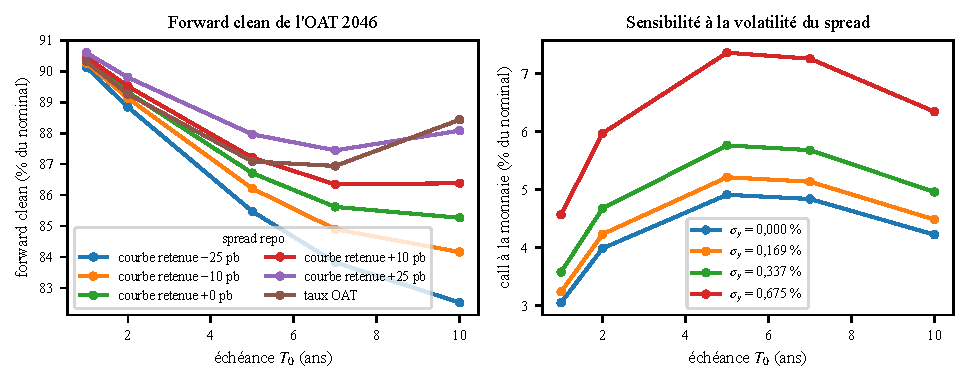
\includegraphics[width=\textwidth]{sensibilites}
\caption{À gauche, forward clean de l'OAT 2046 selon la courbe repo ; à droite, call à la monnaie selon la
volatilité du spread.}
\label{fig:sensibilites}
\end{figure}

\section*{Conclusion}
\addcontentsline{toc}{section}{Conclusion}

Le mémoire a reconstruit sur des données françaises le modèle G2++ de \citet{BrigoMercurio2006}, dans la lecture
de \citet{Russo} où le second facteur est le spread, pour évaluer une option vanille collatéralisée sur l'OAT
4,10~\% 2046 dont le forward est fixé par le repo. Le modèle est recentré sur ce forward comme il est recalé sur
les courbes, et l'option a un prix exact, validé par un Monte-Carlo sans discrétisation.

\subsection*{Réponses aux hypothèses}

L'hypothèse H1 est rejetée. La courbe OAT étant recalée par construction, la procédure de calibration de
\citet{Russo} ne mesure que la convexité de la courbe ; son optimum exact ($\rho = -1$, $a_y = a_x$,
$\sigma_y = \sigma_x$) rend le taux OAT déterministe, et elle ne peut identifier aucun paramètre du spread.

L'hypothèse H2 est confirmée pour la mesure de pricing et rejetée pour la mesure historique. La structure par
terme des volatilités du spread, comme la coupe des spreads dans le filtre de Kalman, identifie une vitesse de
retour risque-neutre quasi nulle ; la GMM estime $\sigma_y$ à 33,7~pb par an et $\rho$ à 0,13, le filtre de Kalman
33,1~pb et 0,15. Mais $\rho$ varie de 0,06 à 0,43 selon le tenor et la fenêtre, bien au-delà de son écart-type, six
ans de données ne suffisent pas à identifier la dynamique historique, et les tests de Hansen et de Ljung-Box
rejettent le spread à un facteur. Les deux régimes de volatilité, de 23 et 51~pb par an, sont trop courts pour
peser sur le prix.

L'hypothèse H3 est confirmée : le facteur spread renchérit le call à la monnaie de 17~\% à toutes les échéances,
et les volatilités réalisées des taux à vingt ans confirment cet ordre de grandeur (rapport OAT~/~€STR de 1,17 dans
les données et de 1,18 dans le modèle).

L'hypothèse H4 est rejetée avec les paramètres estimés. Les deux vitesses de retour étant quasi nulles, un
Hull-White à un facteur sur la courbe OAT, à la volatilité totale du taux OAT, reproduit le call à la monnaie à
1,9~\% près, et, à volatilité ajustée, les prix de 90 à 110~\% du forward à 0,05~\% près. Ce qui compte pour une
option sur une OAT est le niveau de cette volatilité, supérieur de 15~\% à celui que donnent les swaptions €STR ;
sa mesure demande l'historique du spread, faute d'options sur OAT.

L'hypothèse H5 est confirmée à la monnaie et rejetée en dehors. L'approximation à poids gelés ne s'écarte que de
0,12~\% du prix exact à la monnaie lorsque les poids sont gelés à leur valeur forward recentrée ; en dehors, elle
coûte jusqu'à $-3{,}0\,\%$ sur le call à 110~\% et $+4{,}3\,\%$ sur le put à 90~\%, à un an. Le pricer utilise donc le
prix exact.

À la question posée en introduction, la réponse est donc nuancée. Il faut mesurer la volatilité du spread, qui
renchérit l'option de 17~\%, et les séries historiques permettent de l'identifier sous la mesure de pricing. Mais
pour une option sur une seule OAT, un facteur de volatilité augmentée suffit à la représenter. Enfin, aux longues
échéances, le prix dépend autant du niveau du financement en repo que du facteur spread : à dix ans, translater la
courbe repo de $-25$ à $+25$~pb déplace le call à la monnaie de $-21\,\%$ à $+24\,\%$.

\subsection*{Limites}

La première limite est la courbe repo, fictive faute de cotations. Les options sont limitées à dix ans pour que
cette courbe couvre toutes les échéances sans extrapolation ; une courbe de marché à ces durées reposerait
elle-même sur un repo à terme peu liquide. Le recentrage $\delta$ place par ailleurs dans la moyenne du prix une
perte anticipée que sa dispersion ignore. L'approximation reste limitée tant que $\delta$ est petit, 33~pb au plus
ici, mais elle grandirait avec l'écart entre le spread repo et le spread de l'OAT.

Le modèle ne comporte qu'un facteur par courbe, et les tests de Hansen et de Ljung-Box rejettent cette structure :
un seul facteur ne reproduit ni les déformations de pente du spread (deuxième composante principale, 8~\% de la
variance), ni des corrélations qui varient d'un tenor à l'autre. Le spread gaussien peut devenir négatif, ce qui
n'est pas absurde pour un spread OAT–€STR, négatif à deux ans presque tout au long de 2021 et 2022. Seule une
composante de crédit devrait rester positive ; un processus affine positif \citep[cours~1]{MPR2025} l'imposerait.
Le spread, qui mêle crédit, liquidité et effets d'offre, est traité comme un facteur de risque de marché : le modèle
ne décrit pas un événement de crédit sur l'État français.

La calibration est mixte : la volatilité des taux est implicite, celles du spread et la corrélation sont
historiques. Les deux sources sont compatibles sur 2021-2026 pour les taux, sans garantie qu'elles le restent, et
pour le spread l'égalité des volatilités sous les deux mesures reste une hypothèse. La volatilité des taux est
constante ; pour une option européenne, seule compte la variance intégrée jusqu'à l'échéance, et l'effet d'une
volatilité dépendant du temps est borné par les résidus de la diagonale, 2,3~pb au plus. Les conventions sont
simplifiées (base ACT/365 sans calendrier, tenors intermédiaires interpolés, rendements génériques de pair pris
comme taux zéro). Enfin, le modèle gaussien impose sa forme aux prix hors de la monnaie, qu'aucun paramètre ne
permet d'ajuster \citep[section~6.3.5]{Chaix2021}.

\subsection*{Prolongements}

Le premier prolongement est de remplacer la courbe repo fictive par une courbe de marché, au même format. Les
résidus du filtre de Kalman réclament un facteur de pente par courbe et des erreurs de mesure autocorrélées.
L'instabilité de $\rho$, que les régimes de volatilité n'expliquent pas, appellerait une corrélation stochastique,
par exemple un processus autorégressif de Wishart \citep[cours~4, slides~115-118]{MPR2025}, et un G2++ à
changement de régime, qui reste affine (cours~4, slides~44-45), traiterait des options plus courtes que les
régimes. On pourrait aussi séparer une composante de crédit positive et une composante de liquidité, comme
\citet{MonfortRenne2014}, ou introduire une prime de risque de variance sur le spread (cours~6, slides~116-118),
identifiable si des options sur OAT devenaient liquides. Enfin, la structure à deux facteurs compterait vraiment
pour des produits sensibles à l'écart entre les deux courbes, comme les options sur spread ou sur plusieurs titres.

\subsection*{Recul sur la démarche}

Trois enseignements dépassent le cas étudié. Le premier est de tester l'identification avant d'estimer : la
procédure de calibration du papier de référence paraissait naturelle, mais une ligne de calcul montre qu'elle ne
mesure que la convexité de la courbe, et sa mise en œuvre aurait produit des paramètres sans contenu. Le deuxième
est que la définition du contrat compte autant que le modèle : le forward repo, imposé par la pratique de marché,
déplace le prix à dix ans autant que le second facteur. Le troisième est qu'un modèle plus riche n'est utile que
si le produit est sensible à ce qu'il ajoute ; ici, le second facteur se résume, pour le prix, à un supplément de
volatilité, et c'est la mesure de ce supplément qui demande le plus de travail économétrique.
\acompleter{apport du stage pour l'élève et prise de recul personnelle, en quelques phrases}.


\newpage
\renewcommand{\refname}{Bibliographie}
\begin{spacing}{1.15}
\begin{thebibliography}{99}
\addcontentsline{toc}{section}{Bibliographie}
\small

\bibitem[Altonji et Segal(1996)]{AltonjiSegal1996}
Altonji, J. G. et L. M. Segal (1996). Small-Sample Bias in GMM Estimation of Covariance Structures.
\emph{Journal of Business \& Economic Statistics}, 14(3), 353-366.

\bibitem[Brigo et Mercurio(2006)]{BrigoMercurio2006}
Brigo, D. et F. Mercurio (2006). \emph{Interest Rate Models — Theory and Practice. With Smile, Inflation and
Credit}, 2\textsuperscript{e} édition. Springer.

\bibitem[Chaix(2021)]{Chaix2021}
Chaix, A., avec la participation de R. Guillemot (2021). \emph{Modèles de la courbe des taux d'intérêt,
1\textsuperscript{re} partie — Produits dérivés de taux : méthodes d'évaluation et de couverture}. Support de
cours, ENSAE Paris.

\bibitem[Chen et Scott(1993)]{ChenScott1993}
Chen, R.-R. et L. Scott (1993). Maximum Likelihood Estimation for a Multifactor Equilibrium Model of the Term
Structure of Interest Rates. \emph{Journal of Fixed Income}, 3(3), 14-31.

\bibitem[Duffie et Singleton(1999)]{DuffieSingleton1999}
Duffie, D. et K. J. Singleton (1999). Modeling Term Structures of Defaultable Bonds. \emph{Review of Financial
Studies}, 12(4), 687-720.

\bibitem[Engle(1982)]{Engle1982}
Engle, R. F. (1982). Autoregressive Conditional Heteroscedasticity with Estimates of the Variance of United
Kingdom Inflation. \emph{Econometrica}, 50(4), 987-1007.

\bibitem[Hamilton(1989)]{Hamilton1989}
Hamilton, J. D. (1989). A New Approach to the Economic Analysis of Nonstationary Time Series and the Business
Cycle. \emph{Econometrica}, 57(2), 357-384.

\bibitem[Hansen(1982)]{Hansen1982}
Hansen, L. P. (1982). Large Sample Properties of Generalized Method of Moments Estimators. \emph{Econometrica},
50(4), 1029-1054.

\bibitem[Hillairet(2026)]{Hillairet2026}
Hillairet, C. (2026). \emph{Risque de taux}. CM1 : Les taux de marché et la construction de la courbe ; CM2 :
Modèles sur le taux court ; CM3 : Heath-Jarrow-Morton et probabilité forward. Support de cours, ENSAE Paris.

\bibitem[Hull et White(1990)]{HullWhite1990}
Hull, J. et A. White (1990). Pricing Interest-Rate-Derivative Securities. \emph{Review of Financial Studies},
3(4), 573-592.

\bibitem[Jamshidian(1989)]{Jamshidian1989}
Jamshidian, F. (1989). An Exact Bond Option Formula. \emph{Journal of Finance}, 44(1), 205-209.

\bibitem[Kim(1994)]{Kim1994}
Kim, C.-J. (1994). Dynamic Linear Models with Markov-Switching. \emph{Journal of Econometrics}, 60(1-2), 1-22.

\bibitem[Künsch(1989)]{Kunsch1989}
Künsch, H. R. (1989). The Jackknife and the Bootstrap for General Stationary Observations. \emph{Annals of
Statistics}, 17(3), 1217-1241.

\bibitem[Ljung et Box(1978)]{LjungBox1978}
Ljung, G. M. et G. E. P. Box (1978). On a Measure of Lack of Fit in Time Series Models. \emph{Biometrika}, 65(2),
297-303.

\bibitem[Monfort, Pegoraro et Renne(2025)]{MPR2025}
Monfort, A., F. Pegoraro et J.-P. Renne (2025). \emph{Econometrics of Commodity and Asset Pricing}, cours~1 à~6.
ENSAE Paris. Cours cités : 1, Discrete-Time Affine Processes ; 2, Forwards, Futures, Dividends and Convenience
Yields ; 3, Gaussian Affine Term Structure Models ; 4, Switching Regimes and Non-Negative ATSMs ; 5, Estimation of
Affine Asset-Pricing Models, Pricing Credit and Liquidity Risks ; 6, Asset Pricing with Second-Order Esscher
Transform.

\bibitem[Monfort et Renne(2014)]{MonfortRenne2014}
Monfort, A. et J.-P. Renne (2014). Decomposing Euro-Area Sovereign Spreads: Credit and Liquidity Risks.
\emph{Review of Finance}, 18(6), 2103-2151.

\bibitem[Nelson et Siegel(1987)]{NelsonSiegel1987}
Nelson, C. R. et A. F. Siegel (1987). Parsimonious Modeling of Yield Curves. \emph{Journal of Business}, 60(4),
473-489.

\bibitem[Russo et Fabozzi(2016)]{RussoFabozzi2016}
Russo, V. et F. J. Fabozzi (2016). Pricing Coupon Bond Options and Swaptions under the One-Factor Hull-White
Model. \emph{Journal of Fixed Income}, 25, 76-82.

\bibitem[Russo et~al.(s.~d.)]{Russo}
Russo, V., R. Giacometti et F. J. Fabozzi (s.~d.). Closed-Form Solution for Defaultable Bond Options under a
Two-Factor Gaussian Model for Risky Rates Modeling. Document de travail.

\bibitem[Svensson(1994)]{Svensson1994}
Svensson, L. E. O. (1994). Estimating and Interpreting Forward Interest Rates: Sweden 1992-1994. \emph{NBER
Working Paper} 4871.

\end{thebibliography}
\end{spacing}


\newpage
\appendix
\section*{Annexes}
\addcontentsline{toc}{section}{Annexes}
\renewcommand{\thesubsection}{\Alph{subsection}}
\setcounter{subsection}{0}
\renewcommand{\theequation}{\Alph{subsection}.\arabic{equation}}

\subsection{Moments gaussiens du modèle}
\label{ann:moments}
\setcounter{equation}{0}

Notons $(z_1, z_2) = (x, y)$, de paramètres $(a_1, \sigma_1) = (a_x, \sigma_x)$ et $(a_2, \sigma_2) = (a_y, \sigma_y)$,
avec $\rho_{12} = \rho$ et $\rho_{11} = \rho_{22} = 1$. Avec $\tau = T - t$ et $H_a = H_a(t,T)$, les moments
conditionnels à $\F_t$ utilisés aux sections~\ref{sec:modele} à~\ref{sec:resultats} sont, pour $i, j \in \{1, 2\}$ :
\begin{align}
\Cov\big(z_i(T), z_j(T)\big) &= \rho_{ij}\sigma_i\sigma_j\,\frac{1-e^{-(a_i+a_j)\tau}}{a_i+a_j}, \\
\Cov\Big(z_i(T), \int_t^T z_j\Big) &= \frac{\rho_{ij}\sigma_i\sigma_j}{a_j}\Big[\frac{1-e^{-a_i\tau}}{a_i} - \frac{1-e^{-(a_i+a_j)\tau}}{a_i+a_j}\Big], \\
\Cov\Big(\int_t^T z_i, \int_t^T z_j\Big) &= \frac{\rho_{ij}\sigma_i\sigma_j}{a_ia_j}\Big[\tau - H_{a_i} - H_{a_j} + \frac{1-e^{-(a_i+a_j)\tau}}{a_i+a_j}\Big].
\end{align}
Pour $i = j$, la troisième expression redonne $V_{a,\sigma}$, et, pour $i \neq j$, deux fois cette covariance est le
terme croisé $V_{xy}$. Les écarts-types et la corrélation de $(x(T_0), y(T_0))$ qui entrent dans le prix
exact~\eqref{eq:prix_exact} sont $s_x^2 = \Var x(T_0)$, $s_y^2 = \Var y(T_0)$ et
$r_{xy} = \Cov(x(T_0), y(T_0))/(s_xs_y)$, calculés en $t = 0$.

\paragraph{Moyennes sous la mesure forward.} D'après~\eqref{eq:zc_hw}, le numéraire $P(u,T_0)$ a pour
volatilité $-\sigma_x H_{a_x}(u,T_0)$, portée par le seul brownien $W_x$. Le changement de numéraire donne
\begin{equation}
\dd W_x^{T_0} = \dd W_x + \sigma_x H_{a_x}(u,T_0)\,\dd u,\qquad
\dd W_y^{T_0} = \dd W_y + \rho\,\sigma_x H_{a_x}(u,T_0)\,\dd u.
\end{equation}
En intégrant la dynamique~\eqref{eq:dynamique} de $0$ à $T_0$, il vient
\begin{equation}
\begin{split}
\mu_x &= -\int_0^{T_0}\sigma_x^2 H_{a_x}(u,T_0)\,e^{-a_x(T_0-u)}\,\dd u = -\Cov\Big(x(T_0),\int_0^{T_0}x\Big),\\
\mu_y &= -\int_0^{T_0}\rho\,\sigma_x\sigma_y H_{a_x}(u,T_0)\,e^{-a_y(T_0-u)}\,\dd u = -\Cov\Big(y(T_0),\int_0^{T_0}x\Big),
\end{split}
\end{equation}
dont les expressions fermées sont celles de la section~\ref{sec:evaluation}.

\subsection{Prix des options}
\label{ann:prix}

\begin{table}[H]
\centering\small
\caption{Calls et puts sur l'OAT 4,10~\% 2046, modèle à deux facteurs, prix exacts pour 100 de nominal (strike
clean en \% du forward clean)}
\label{tab:prix_complets}
\begin{tabular}{@{}lrrrrr@{}}
\toprule
Strike & 1 an & 2 ans & 5 ans & 7 ans & 10 ans \\
\midrule
\multicolumn{6}{@{}l}{\emph{Calls}} \\
90~\%  & 9,434 & 9,837 & 9,961 & 9,514 & 8,442 \\
95~\%  & 6,099 & 6,951 & 7,660 & 7,421 & 6,539 \\
100~\% & 3,578 & 4,677 & 5,763 & 5,679 & 4,960 \\
105~\% & 1,899 & 3,000 & 4,248 & 4,271 & 3,689 \\
110~\% & 0,914 & 1,840 & 3,073 & 3,161 & 2,695 \\
\midrule
\multicolumn{6}{@{}l}{\emph{Puts}} \\
90~\%  & 0,641 & 1,398 & 2,475 & 2,577 & 2,206 \\
95~\%  & 1,703 & 2,732 & 3,917 & 3,952 & 3,421 \\
100~\% & 3,578 & 4,677 & 5,763 & 5,679 & 4,960 \\
105~\% & 6,296 & 7,220 & 7,990 & 7,740 & 6,807 \\
110~\% & 9,707 & 10,279 & 10,558 & 10,099 & 8,931 \\
\midrule
\multicolumn{6}{@{}l}{\emph{Forward et espérance du modèle (prix dirty)}} \\
$F$ (repo) & 91,573 & 90,525 & 87,908 & 86,809 & 86,445 \\
$M$ (non recentré) & 91,267 & 90,172 & 87,824 & 87,516 & 88,742 \\
\bottomrule
\end{tabular}
\end{table}

\subsection{Ajustement de la courbe OAT}
\label{ann:oat}

\begin{table}[H]
\centering\small
\caption{OAT utilisées pour la courbe Nelson-Siegel-Svensson : prix clean au 8 septembre 2026 et résidus en
rendement}
\label{tab:residus_oat}
\begin{tabular}{@{}llccr@{}}
\toprule
ISIN & Maturité & Coupon (\%) & Prix clean & Résidu (pb) \\
\midrule
FR0129570570 & 30/09/2026 & 0,00 & 99,868 & $-0{,}4$ \\
FR0129704112 & 09/12/2026 & 0,00 & 99,372 & 1,4 \\
FR0129704153 & 10/03/2027 & 0,00 & 98,649 & $-1{,}5$ \\
FR0129570646 & 16/06/2027 & 0,00 & 97,849 & 0,7 \\
FR0129704195 & 08/09/2027 & 0,00 & 97,121 & $-0{,}8$ \\
FR001400XLW2 & 24/09/2028 & 2,40 & 98,506 & 0,7 \\
FR0014016G71 & 24/09/2029 & 2,40 & 97,474 & 0,5 \\
FR0013516549 & 25/11/2030 & 0,00 & 86,758 & 1,3 \\
FR0014018OI0 & 25/02/2032 & 3,25 & 98,160 & $-1{,}7$ \\
FR001400BKZ3 & 25/11/2032 & 2,00 & 90,604 & 0,4 \\
FR001400L834 & 25/11/2033 & 3,50 & 97,730 & $-1{,}2$ \\
FR001400QMF9 & 25/11/2034 & 3,00 & 93,115 & $-0{,}6$ \\
FR0014012II5 & 25/11/2035 & 3,50 & 95,405 & 0,1 \\
FR0014018YR0 & 25/11/2036 & 3,70 & 95,759 & 0,0 \\
FR001400WYO4 & 25/05/2042 & 3,60 & 88,794 & 2,8 \\
\textbf{FR0014015MU5} & \textbf{25/05/2046} & \textbf{4,10} & \textbf{91,690} & \textbf{2,0} \\
FR0013404969 & 25/05/2050 & 1,50 & 53,283 & 8,4 \\
FR0014016CV2 & 25/05/2057 & 4,40 & 90,960 & $-14{,}5$ \\
FR0014001NN8 & 25/05/2072 & 0,50 & 22,699 & 3,2 \\
\midrule
\multicolumn{5}{@{}l}{\footnotesize Erreur quadratique moyenne : 4,1~pb. En gras, le sous-jacent des options.} \\
\bottomrule
\end{tabular}
\end{table}

\subsection{Environnement de calcul}
\label{ann:calcul}

Les calculs sont regroupés dans un notebook Jupyter unique, \nolinkurl{main/oat_option_pricer.ipynb}, écrit en
Python~3.12 ; l'environnement est figé par le gestionnaire \texttt{uv} (fichiers \texttt{pyproject.toml} et
\texttt{uv.lock}). Les bibliothèques utilisées sont NumPy et SciPy (optimisation, quadrature de Gauss-Hermite,
splines), pandas, matplotlib, statsmodels (filtre de Kalman par la classe \texttt{MLEModel}, régression à
changement de régime \texttt{MarkovRegression}, tests ARCH-LM et de Ljung-Box), scikit-learn (analyse en
composantes principales) et joblib (parallélisation du test sur données simulées). L'exécution complète du
notebook prend environ une minute et quinze secondes. Les données de marché sont lues dans le fichier Bloomberg
\nolinkurl{data/market data bloom.xlsx} et la courbe repo fictive dans \nolinkurl{data/repo_fictif.csv} ; une courbe de
marché s'y substituerait au même format. Les figures de ce rapport sont produites par le script
\nolinkurl{memoire/figures/generer_figures.py}, qui exécute le notebook sans modifier ses calculs.


\newpage
\section*{Note de synthèse}
\addcontentsline{toc}{section}{Note de synthèse}

\textbf{Cadre.} Ce travail a été mené pendant le stage de fin d'études réalisé chez
\acompleter{nom de l'entreprise}, au sein de \acompleter{équipe}, du \acompleter{dates}. Il porte sur
l'évaluation d'options sur obligations d'État françaises, les OAT. Une option d'achat (call) donne le droit
d'acheter l'obligation à une date future à un prix fixé aujourd'hui ; une option de vente (put), celui de la
vendre. Le contrat étudié est celui qui se traite en banque. L'option est garantie par un dépôt de collatéral
rémunéré au taux interbancaire au jour le jour €STR, et son prix à terme se déduit du coût de financement du titre
sur le marché de la pension livrée (repo).

\textbf{Problématique.} Le prix d'une OAT dépend de deux sources de risque : le niveau des taux sans risque, et
l'écart (spread) entre le rendement de l'OAT et ces taux, qui rémunère le risque de crédit de l'État, la liquidité
du titre et des effets d'offre. Les modèles de taux usuels ne retiennent que la première source. Or il n'existe pas
de marché d'options sur OAT d'où l'on pourrait tirer la volatilité du spread. La question posée est double :
faut-il modéliser le spread comme un risque à part pour évaluer une option sur OAT, et les données disponibles
permettent-elles d'en mesurer les caractéristiques ?

\textbf{Démarche.} Le modèle retenu, issu de la littérature (Brigo et Mercurio, 2006 ; Russo, Giacometti et
Fabozzi), décrit le taux de l'OAT comme la somme de deux facteurs aléatoires gaussiens : le taux sans risque et le
spread. Le facteur taux est calibré sur les prix des swaptions, options sur taux d'intérêt très liquides. Pour le
facteur spread, on montre d'abord que la méthode proposée dans l'article de référence, fondée sur la seule courbe
des taux OAT, ne peut rien mesurer. Les paramètres du spread sont donc estimés sur six ans de données
quotidiennes (2021-2026), par deux méthodes économétriques enseignées à l'ENSAE : la méthode des moments
généralisée et le maximum de vraisemblance avec filtre de Kalman. Le prix de l'option est calculé exactement, et
ce calcul est validé par simulation de Monte-Carlo. Les données proviennent de Bloomberg (8 septembre 2026), et
l'option porte sur l'OAT 4,10~\% 2046, pour des échéances de un à dix ans.

\textbf{Résultats.} Quatre résultats se dégagent.
\begin{itemize}
\item La volatilité du spread est d'environ 34 points de base par an, sa corrélation avec les taux de 0,13 ;
elle alterne entre une période calme (23 points de base) et des épisodes agités (51 points de base), comme
en 2022 ou lors des crises politiques de 2024, mais ces épisodes sont trop courts pour modifier le prix.
\item Prendre en compte le spread renchérit l'option de 17~\%, à toutes les échéances.
\item Cet effet se résume, pour une option sur une seule OAT, à une volatilité augmentée : un modèle à un seul
facteur, dont la volatilité est relevée d'environ 17~\%, reproduit les prix à 0,05~\% près.
\item La formule approchée de l'article de référence est précise pour les options à la monnaie, mais commet des
erreurs de 3 à 4~\% sur les options éloignées de la monnaie : le prix exact est préférable.
\end{itemize}
Enfin, pour les échéances longues, le coût de financement en repo pèse autant sur le prix que le spread lui-même.

\textbf{Limites et suites.} Faute de cotations, la courbe de financement en repo utilisée est fictive ; une courbe
de marché la remplacerait sans modifier les calculs. Les tests statistiques montrent qu'un seul facteur par courbe
ne décrit pas toutes les déformations du spread, et la corrélation entre spread et taux est instable dans le
temps. Ces points ouvrent la voie à des modèles plus riches, utiles surtout pour des produits sensibles à l'écart
entre plusieurs obligations.

\newpage
\begin{otherlanguage}{english}
\section*{Executive summary}
\addcontentsline{toc}{section}{Executive summary}

\textbf{Context.} This work was carried out during the end-of-studies internship at
\acompleter{company name}, in \acompleter{team}, from \acompleter{dates}. It deals with the valuation of options on
French government bonds (OATs). A call option gives the right to buy the bond at a future date for a price fixed
today; a put option gives the right to sell it. The contract studied is the one traded by banks: the option is
collateralised, with collateral paid at the €STR overnight rate, and its forward price follows from the cost of
financing the bond in the repurchase (repo) market.

\textbf{Research question.} The price of an OAT depends on two sources of risk: the level of risk-free rates, and
the spread between the OAT yield and those rates, which compensates for the credit risk of the French State, the
liquidity of the bond and supply effects. Standard interest rate models only capture the first source, and there
is no liquid market for OAT options from which the volatility of the spread could be inferred. The question is
therefore twofold: should the spread be modelled as a separate risk factor to price an OAT option, and can its
parameters be identified from the available data?

\textbf{Approach.} The model, taken from the literature (Brigo and Mercurio, 2006; Russo, Giacometti and Fabozzi),
describes the OAT short rate as the sum of two Gaussian factors: the risk-free rate and the spread. The rate factor
is calibrated to swaption prices, which are very liquid interest rate options. For the spread factor, we first
show that the calibration procedure proposed in the reference paper, based on the OAT yield curve alone, cannot
identify any parameter. The spread parameters are therefore estimated on six years of daily data (2021-2026),
with two econometric methods taught at ENSAE: the generalised method of moments and maximum likelihood with the
Kalman filter. The option price is computed exactly, and the computation is validated by Monte Carlo simulation.
Market data come from Bloomberg (8 September 2026); the option is written on the 4.10\% OAT maturing in 2046, with
expiries from one to ten years.

\textbf{Results.} Four results stand out.
\begin{itemize}
\item The volatility of the spread is about 34 basis points per year and its correlation with rates is 0.13; it
switches between a calm regime (23 basis points) and turbulent episodes (51 basis points), such as 2022 or the
French political crises of 2024, but these episodes are too short to affect the price.
\item Accounting for the spread makes the option 17\% more expensive, at all expiries.
\item For an option on a single OAT, this effect amounts to a higher volatility: a one-factor model whose
volatility is raised by about 17\% reproduces the prices within 0.05\%.
\item The closed-form approximation of the reference paper is accurate for at-the-money options but errs by 3
to 4\% for options far from the money: the exact price should be preferred.
\end{itemize}
Finally, for long expiries, the repo financing cost weighs as much on the price as the spread itself.

\textbf{Limitations and extensions.} For lack of quotes, the repo curve used is fictitious; a market curve would
replace it without changing the computations. Statistical tests show that a single factor per curve does not
capture all the deformations of the spread, and that the correlation between spread and rates is unstable over
time. These findings call for richer models, mostly relevant for products sensitive to the spread between
several bonds.
\end{otherlanguage}


\end{document}
